\documentclass[journal]{IEEEtran}
% IEEE Transactions journal format (IEEEtran.cls v1.8b). Compile: pdflatex, bibtex, pdflatex, pdflatex.
\usepackage{cite}
\usepackage{amsmath,amssymb}
\usepackage{graphicx}
\usepackage{booktabs}
\usepackage{multirow}
\usepackage{array}
\usepackage{url}
\usepackage{xr}
\externaldocument[S-]{supplement}
\usepackage[hidelinks]{hyperref}
\graphicspath{{figures/}}
\renewcommand{\topfraction}{0.92}\renewcommand{\bottomfraction}{0.6}\renewcommand{\textfraction}{0.06}
\renewcommand{\floatpagefraction}{0.8}\renewcommand{\dbltopfraction}{0.92}\renewcommand{\dblfloatpagefraction}{0.8}
\setcounter{totalnumber}{6}\setcounter{topnumber}{4}\setcounter{dbltopnumber}{3}
\hyphenation{Dino-Bloom Efficient-Net cyto-morphology}
\newcommand{\Ccontrib}[1]{\textsf{C#1}}

\begin{document}

\title{Leakage-Aware, Sensitivity-First Validation of Blood-Smear Leukemia Classifiers: A Two-Dataset Study of Engineered Features, Deep Features and Dimensionality Reduction}

\author{First~Author and Second~Author% <-- replace with the authors' names
\thanks{Manuscript received XX; revised XX. (Corresponding author: First Author.)}%
\thanks{First Author is with [Department], [Institution], [City], [Country] (e-mail: [e-mail]).}%
\thanks{Second Author is with [Department], [Institution], [City], [Country] (e-mail: [e-mail]).}}

\markboth{IEEE Transactions on [Journal Name], Vol.~XX, No.~XX, 2026}%
{Author \MakeLowercase{\textit{et al.}}: Leakage-Aware, Sensitivity-First Validation of Blood-Smear Leukemia Classifiers}

\maketitle

\begin{abstract}
Deep-learning models for leukemia detection in blood smears often report 97--100\% accuracy, yet few are used in practice. We examined how much of this performance survives on new patients, using two public datasets: 106 patients with acute myeloid leukemia (34 with acute promyelocytic leukemia, APL) split by diagnosis date, and C-NMC 2019 (73 subjects, acute lymphoblastic leukemia vs.\ normal B cells) with a held-out fold. The same models reached 88--95\% accuracy when cells of one patient could appear in both training and test sets, but 69--90\% on new patients, and the area under the ROC curve (AUROC) was inflated by up to 0.32 when cells carried the patient's diagnosis. Guided by an exploratory analysis that found a stain shift in the APL cohort only, we compared preprocessing options, engineered, frozen and fine-tuned convolutional features, principal component analysis (PCA), early stopping and attention pooling, reporting every step before and after. A pre-specified pipeline---Macenko stain normalization, a fine-tuned network and engineered features combined in an ensemble---detected all 12 APL patients in the later cohort (recall 1.00, AUROC 0.81) at a specificity of 0.17, and 16 of 17 leukemic subjects in C-NMC (AUROC 0.96, specificity 0.79). Fine-tuning was the most consistent improvement; PCA reduced model size 20-fold at a small cost in F1 score (0.79 to 0.76); early stopping and attention pooling gave no gain. A new laboratory needs about 20 confirmed positive cases to recalibrate a decision threshold. We recommend patient-level splits, more than one external test, sensitivity-first reporting and local calibration before clinical use.
\end{abstract}

\begin{IEEEkeywords}
Acute promyelocytic leukemia, acute lymphoblastic leukemia, blood smear, data leakage, deep learning, dimensionality reduction, external validation, feature engineering, multiple instance learning, sensitivity.
\end{IEEEkeywords}

%======================================================================
\section{Introduction}
\IEEEPARstart{A}{cute} leukemia is usually first suspected on a peripheral blood smear, where a trained morphologist looks for blasts and other abnormal white cells \cite{khoury2022who}. Acute promyelocytic leukemia (APL) shows how much rides on that first look: it is a medical emergency, because patients can bleed to death within days unless all-trans retinoic acid is started as soon as APL is suspected, often before genetic confirmation arrives. Reading smears takes time and experience, and the experience is not available everywhere, which is why automated smear analysis has attracted so much work.

Published results look encouraging. Many deep-learning models report accuracies between 97\% and 100\% for leukemia detection from single-cell images \cite{jammal2025causalformer,jammal2025neurobridge}, and weakly supervised models reach AUCs above 0.95 for recognizing APL \cite{manescu2023apl}. Yet few of these systems are used in practice. Our starting point is that part of the gap lies not in the models but in how they are evaluated. When cells from the same patient appear in both the training and test sets, a model can succeed by recognizing the patient---the stain, the smear, the day it was scanned---rather than the disease. When the label is the patient's diagnosis copied onto every cell, this shortcut is always available. And when performance is summarized by accuracy alone, it hides the error that matters most clinically: a sick patient called healthy. Similar leakage and shortcut problems have been documented across machine-learning-based science \cite{kapoor2023leakage} and in medical imaging \cite{zech2018confounding,roberts2021pitfalls}.

In this work we measure these effects directly on a public cohort of 106 patients with acute myeloid leukemia (AML), 34 of whom have APL, replicate the analysis on the C-NMC 2019 dataset of acute lymphoblastic leukemia, and build an evaluation that a clinician could trust. Our contributions are:
\begin{itemize}
\item[\Ccontrib{1}] \emph{A controlled leakage audit on two datasets.} With identical data, features and classifiers, we compare image-level cross-validation (CV), patient-grouped CV and an untouched external set, both for a label that belongs to the patient and for a label that belongs to the cell.
\item[\Ccontrib{2}] \emph{External validation of two kinds.} Models are developed on an earlier APL-AML cohort and tested once on patients diagnosed later, and on C-NMC developed on two official folds and tested on the third; a pooled 106-patient analysis adds statistical power.
\item[\Ccontrib{3}] \emph{Sensitivity-first reporting.} Decision thresholds are set on the development cohort for a sensitivity of at least 0.95, and we report recall, the number of missed APL patients, specificity, F1 score, negative predictive value and calibration, not only accuracy and AUROC. We also quantify how many local cases a new laboratory needs to restore the operating point, and the net benefit at a realistic prevalence.
\item[\Ccontrib{4}] \emph{Data-driven design, step by step.} Starting from an exploratory analysis of both datasets, we choose preprocessing with a rule fixed in advance, compare 93 interpretable morphology features with frozen and fine-tuned CNN features, and test PCA, early stopping and attention pooling, reporting every component before and after it is added.
\item[\Ccontrib{5}] \emph{Pre-specified pipelines with their cost.} We fix a primary pipeline and a low-complexity secondary pipeline before the final analysis, both trainable on a CPU and built on attention-based multiple instance learning (MIL) \cite{ilse2018abmil} and fine-tuned features, and report their performance together with storage, model size and time per patient.
\end{itemize}
Code, split files and label maps are released so that results on both datasets can be compared directly in future work.

%======================================================================
\section{Related Work}
Table~\ref{tab:survey} summarizes representative studies. For each, the last column notes an open question that the study was not designed to answer and links it to the contribution of this paper that addresses it.

\subsection{Cell-Level Classification of Blood Smears}
Much of the literature classifies single segmented cells as leukemic or normal. The C-NMC 2019 challenge \cite{gupta2022cnmc} set a useful standard by holding out whole subjects for testing: ResNeXt models reached a weighted F1 score of 0.889 \cite{prellberg2019cnmc}, and a weighted ensemble of five CNNs reached 0.886 with an AUC of 0.941 \cite{mondal2021ensemble}. More recent transformer and hybrid designs report accuracies of 0.97 to 1.00 on C-NMC and on the ALL image dataset \cite{jammal2025causalformer,jammal2025neurobridge}, and hybrid pipelines that feed CNN features to classical classifiers reach 0.88 when separating lymphoblasts, myeloblasts and normal cells \cite{kasim2025multiclass}. These studies advanced architectures and training strategies. Because the split unit is not always reported, and because some of them combine sources in which class and source coincide, it remains open how much of their performance would carry over to new patients (\Ccontrib{1}, \Ccontrib{2}). A recent subject-disjoint benchmark on C-NMC found an AUROC of 0.913 \cite{albzour2026leakage}, which suggests that the split matters, but it covered a single, cell-level label.

\subsection{Patient-Level and Weakly Supervised Diagnosis}
Clinical decisions are made per patient, and several groups have moved in that direction with MIL. Expert-level single-cell classification \cite{matek2019blast,matek2021bmc} made it possible to identify genetic AML subtypes from blood-smear cells \cite{hehr2023scemila} and NPM1 or FLT3-ITD status from marrow \cite{wei2025annotationfree,eckardt2022npm1}. For APL, Sidhom \emph{et al.} \cite{sidhom2021apl} released the cohort used here and showed that a single-cell model trained on the earlier patients reached a cell-level AUC of 0.890 in development and 0.743 in the later validation cohort. Manescu \emph{et al.} \cite{manescu2023apl} trained an annotation-free MIL model on the same patients and reported an AUC of 0.96 under random three-fold CV. Interpretable morphometry has also proved useful: engineered cell features with sparse regression detected myelodysplasia and anemia subtypes and held up in an external cohort \cite{dealmeida2023haemorasis}. Across these studies, the number of missed patients at a clinically chosen operating point and the calibration of predicted probabilities are rarely reported (\Ccontrib{3}), and engineered features have not yet been compared with deep features for acute leukemia under the same protocol (\Ccontrib{4}).

\subsection{Foundation Models and Generalization}
Hematology foundation models aim to make cell representations robust to scanners and stains. DinoBloom, trained on more than 380,000 cells from 13 datasets, outperforms generic encoders \cite{koch2024dinobloom}; later work adapts DINOv3 with a risk-aware loss \cite{muminov2025cytodino} and compares foundation models with retrieval under a held-out-dataset protocol \cite{zamora2026retrieval}, while LeukemiaAttri provides images of the same films from different microscopes \cite{rehman2024leukemiaattri}. The largest patient-level study to date trained a DinoBloom-based transformer on 6,610 individuals and validated it on two external sets, including the cohort used here \cite{dasdelen2026caitomorph}. Such models need large labeled cohorts and GPU resources; whether lightweight models trained on a few hundred patients can be evaluated just as rigorously is the question behind \Ccontrib{5}.

\begin{table*}[!t]
\centering
\caption{Representative previous studies. Results are as reported by each study and are not directly comparable across datasets. The last column notes an open question each study was not designed to address and the contribution of this paper (C1--C5) that addresses it.}
\label{tab:survey}
\setlength{\tabcolsep}{3pt}
\renewcommand{\arraystretch}{1.08}
\footnotesize
\begin{tabular}{p{2.3cm}p{2.5cm}p{2.7cm}p{2.8cm}p{2.4cm}p{4.15cm}}
\toprule
Study & Data & Method & Evaluation & Reported result & Open question (addressed by) \\
\midrule
Prellberg \& Kramer, 2019 \cite{prellberg2019cnmc} & C-NMC, ALL vs.\ normal cells & ResNeXt with squeeze-excitation & Challenge test set, unseen subjects & Weighted F1 0.889 & Cell-level only; missed-case rate and calibration not reported (C3, C5) \\
Mondal \emph{et al.}, 2021 \cite{mondal2021ensemble} & C-NMC & Weighted ensemble of five CNNs & Preliminary test set, 28 subjects & F1 0.886; AUC 0.941 & Cell-level only; ensemble cost (C3, C5) \\
Kasim \emph{et al.}, 2025 \cite{kasim2025multiclass} & ALL-IDB2 + AML-LMU, 390 cells & CNN features + SVM/XGBoost & Image-level split & Accuracy 0.88 (3 classes) & Class and source coincide; patient grouping unavailable (C1, C2) \\
Jammal \& Dahab, 2025 \cite{jammal2025causalformer} & C-NMC & CNN--ViT with causal reasoning & Split unit not reported & Accuracy 1.00 & Transfer to new patients unknown (C1, C2) \\
Jammal \emph{et al.}, 2025 \cite{jammal2025neurobridge} & ALL image; C-NMC & Neuro-symbolic ViT & 5-fold CV, split unit not reported & Accuracy 1.00; 0.97 & Transfer to new patients unknown (C1, C2) \\
Albzour, 2026 \cite{albzour2026leakage} & C-NMC & ML, CNN and ViT benchmark & Subject-disjoint, unseen subjects & AUROC 0.913 & One cell-level label; no patient-level model (C1, C5) \\
Matek \emph{et al.}, 2019 \cite{matek2019blast} & AML-LMU, 200 patients & ResNeXt & Single-cell test set & Expert-level on 15 cell types & Single centre; diagnosis per patient not addressed (C2, C5) \\
Hehr \emph{et al.}, 2023 \cite{hehr2023scemila} & 189 patients, 4 AML subtypes & Attention MIL & Patient-level CV & Subtype identification & Single laboratory; operating point not reported (C2, C3) \\
Sidhom \emph{et al.}, 2021 \cite{sidhom2021apl} & APL-AML, 106 patients (\emph{this cohort}) & Single-cell CNN + MIL & Temporal validation & Cell AUC 0.890 $\rightarrow$ 0.743 & Missed APL patients and calibration not reported (C3) \\
Manescu \emph{et al.}, 2023 \cite{manescu2023apl} & APL-AML (\emph{this cohort}) and others & Annotation-free MIL (VGG-19) & Random 3-fold CV & AUC 0.96 & Random rather than temporal split (C1, C2) \\
de Almeida \emph{et al.}, 2023 \cite{dealmeida2023haemorasis} & 352 + 63 slides & Engineered morphometry + glmnet / MIL & Cross-validation and external cohort & Up to 0.90 AUC (MDS subtype) & Not applied to acute leukemia (C4) \\
Wei \emph{et al.}, 2025 \cite{wei2025annotationfree} & 572 marrow slides & MIL ensemble & Single-centre test cohort & NPM1 AUC 0.90 & External cohort not available (C2) \\
Koch \emph{et al.}, 2024 \cite{koch2024dinobloom} & 13 datasets, 380k cells & DINOv2 foundation model & Linear probing, MIL & Outperforms generic encoders & Patient-level external evaluation open (C2, C5) \\
Dasdelen \emph{et al.}, 2026 \cite{dasdelen2026caitomorph} & 6,610 individuals; external incl.\ this cohort & DinoBloom + transformer MIL & Two external sets & 8-class acc.\ 0.72; malignancy AUC 0.97 & Needs large cohort and GPU (C5) \\
Zamora \emph{et al.}, 2026 \cite{zamora2026retrieval} & Five datasets & Foundation models + retrieval & Held-out dataset & --- & Patient leakage not separated from dataset shift (C1) \\
\bottomrule
\end{tabular}
\end{table*}

%======================================================================
\section{Materials and Methods}

\subsection{Dataset}
We used the public APL-AML cohort of Sidhom \emph{et al.} \cite{sidhom2021apl}. It contains single-cell images from Wright-stained peripheral blood smears of 106 adults with AML treated at Johns Hopkins Hospital between 2010 and 2020, captured with a CellaVision DM100 analyzer. Thirty-four patients have APL and 72 have other AML subtypes. The authors split the cohort by date: 82 patients diagnosed before January 2019 form the Discovery cohort and 24 diagnosed later form the Validation cohort. The 25,724 cell images measure about $360\times363$ pixels; 15,632 of them carry a cell type assigned by the analyzer and confirmed by its operator, and the remaining 10,092 are unlabeled. Table~\ref{tab:dataset} and Fig.~\ref{fig:dataset} describe the composition.

\begin{table}[!t]
\centering
\caption{Composition of the APL-AML cohort.}
\label{tab:dataset}
\resizebox{\columnwidth}{!}{%
\begin{tabular}{llrrrr}
\toprule
Cohort & Diagnosis & Patients & Cells & Labeled cells & Cells per patient \\
 & & & & & median (range) \\
\midrule
Discovery & AML & 60 & 11,523 & 8,077 & 134 (98--984) \\
 & APL & 22 & 8,764 & 4,082 & 290 (112--1,066) \\
Validation & AML & 12 & 3,589 & 1,893 & 252 (116--554) \\
 & APL & 12 & 1,848 & 1,580 & 140 (83--268) \\
\midrule
Total & & 106 & 25,724 & 15,632 & 152 (83--1,066) \\
\bottomrule
\end{tabular}}
\end{table}

\begin{figure*}[!t]
\centering
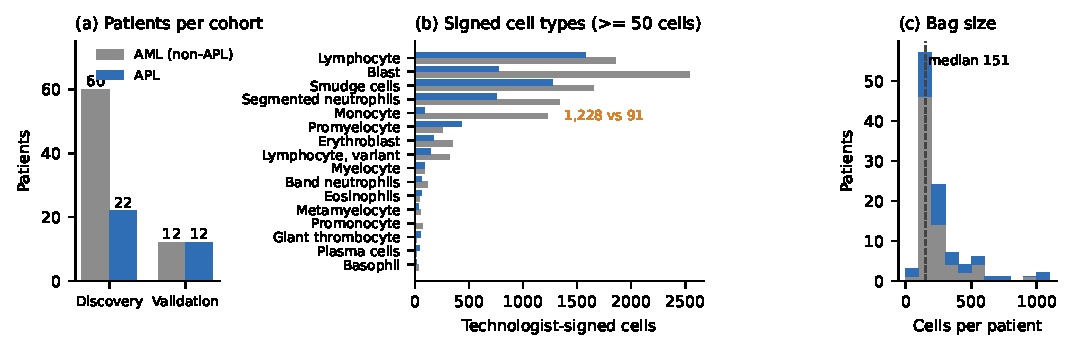
\includegraphics[width=\textwidth]{fig_dataset.pdf}
\caption{Cohort composition. (a) Patients per cohort and diagnosis. (b) Labeled cell types with at least 50 cells; monocytes are almost absent in APL (1,228 vs.\ 91 cells). (c) Number of cells per patient.}
\label{fig:dataset}
\end{figure*}

The cohort has several characteristics that shape the analysis. The classes are imbalanced and the imbalance shifts between cohorts: APL makes up 27\% of Discovery patients but 50\% of Validation patients, so accuracy alone would mean different things in the two cohorts. The number of cells per patient is confounded with the diagnosis in opposite directions---Discovery APL patients have about twice as many cells as AML patients, whereas the reverse holds in Validation---so our patient-level models are designed to be insensitive to bag size. The original authors note that all Discovery smears scanned before 2018 were APL \cite{sidhom2021apl}, which means that acquisition date carries diagnostic information inside the Discovery cohort and invites shortcut learning whenever patients leak across splits. The mix of cell types also differs by diagnosis; labeled monocytes, for example, are nearly absent in APL. Finally, ten image files are truncated, 54 are full microscope fields rather than single-cell crops, cell labels are analyzer classifications verified by an operator rather than consensus annotations, and the Validation cohort comes from the same hospital and contains only 24 patients.

To test whether our findings hold beyond one hospital, we repeated the analyses on a second public dataset, C-NMC 2019 \cite{gupta2022cnmc}, obtained from Kaggle. It contains 10,661 segmented single-cell images ($450\times450$ pixels, cell on a black background) from 73 subjects: 47 with B-lineage acute lymphoblastic leukemia (ALL) and 26 healthy individuals whose normal B cells serve as controls. The images were acquired in a different laboratory, with a different stain and microscope, from the APL-AML cohort. The challenge organizers distributed the training data in three subject-disjoint folds. Before any analysis we designated folds 0 and 1 as the development set (42 subjects, 7,108 cells; 30 with ALL) and fold 2 as the external test set (31 subjects, 3,553 cells; 17 with ALL). Every C-NMC cell is labeled with its subject's diagnosis, so the label belongs to the subject, as in T1 below; unlike the APL-AML cells, however, the ALL cells were selected as malignant lymphoblasts, so the label is also partly a property of the cell.

\subsection{Learning Tasks}
We defined five tasks (Table~\ref{tab:tasks}). In T1 every APL-AML cell inherits its patient's diagnosis, which reproduces a common way of building single-cell datasets. In T2 the label is the cell's own type (blast versus other labeled white cells, excluding artefacts, unidentified cells, smudge cells and platelets). T3 is the clinical question: does this patient have APL? T4 and T5 are the C-NMC counterparts of T1 and T3: classifying single cells, and classifying subjects, as ALL or normal.

\begin{table}[!t]
\centering
\caption{Learning tasks (development / external set). T1--T3: APL-AML (Discovery / Validation); T4, T5: C-NMC 2019 (folds 0--1 / fold 2).}
\label{tab:tasks}
\resizebox{\columnwidth}{!}{%
\begin{tabular}{lllr}
\toprule
Task & Unit & Positive class & Size \\
\midrule
T1 Diagnosis on cells & Cell & Cell from an APL patient (43.2\%) & 20,287 / 5,437 cells \\
T2 Blast detection & Cell & Labeled blast (28.0\%) & 9,694 / 2,863 cells \\
T3 Patient diagnosis & Patient & APL (22 of 82) & 82 / 24 patients \\
\midrule
T4 C-NMC cells & Cell & Cell from an ALL subject (67.7\%) & 7,108 / 3,553 cells \\
T5 C-NMC subjects & Subject & ALL (30 of 42) & 42 / 31 subjects \\
\bottomrule
\end{tabular}}
\end{table}

\subsection{Preprocessing and Cell Segmentation}
Fig.~\ref{fig:preproc} outlines the pipeline. A manifest records every image with its patient, cohort, diagnosis and cell label. Unreadable files are kept as missing rows and imputed inside each training fold, and no image is removed because of its label. The Validation cohort is never used for fitting, threshold selection or calibration.

\begin{figure}[!t]
\centering
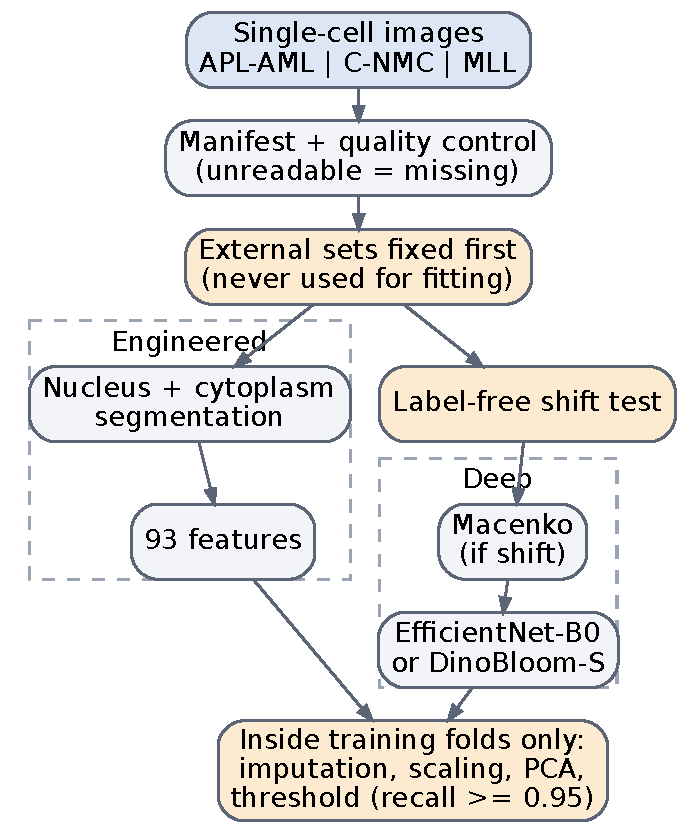
\includegraphics[width=0.92\columnwidth]{fig_preprocessing.pdf}
\caption{Preprocessing pipeline for both datasets. The orange steps prevent leakage: the external sets are fixed before any analysis, and every statistic---imputation, scaling, PCA, class weights and the decision threshold---is fitted inside the training fold.}
\label{fig:preproc}
\end{figure}

For the engineered features, each image is resized to $192\times192$ pixels and separated into hematoxylin, eosin and residual channels by color deconvolution \cite{ruifrok2001deconvolution}. The nucleus is segmented by Otsu thresholding \cite{otsu1979} of the smoothed hematoxylin channel, followed by morphological opening and selection of the component nearest the image center. We found that pale cytoplasm could not be separated reliably from neighboring red cells by color, so instead of claiming a full cell outline we describe the cytoplasm with two proxies: a basophilic region of blue-dominant pixels within one nuclear radius, and a perinuclear ring 2--9 pixels wide that excludes the bright background (Fig.~\ref{S-fig:seg}). C-NMC cells are already segmented and lie on a black background, which the stain-based nucleus segmentation would read as dense chromatin. For C-NMC we therefore set pixels whose brightest channel is below 15 to white before extracting engineered features, so that the same segmentation applies; the CNN received the original images.

The exploratory analysis (Section~\ref{sec:eda}) showed that stain and color differed between the APL-AML cohorts. We therefore compared four ways of preparing images for the CNN---no preprocessing, edge sharpening (unsharp mask), Reinhard color normalization \cite{reinhard2001color} and Macenko stain normalization \cite{macenko2009stain}---and fixed the selection rule in advance: the method had to reduce the measurable cohort shift without lowering external performance. Macenko normalization estimates the two stain directions of each image in optical-density space and maps them, and their concentrations, onto reference stains. Because smear backgrounds are beige rather than white, we estimated the illumination of each image from the 99th percentile of each color channel instead of assuming a white background, and we estimated the reference stains from 300 Discovery images only. Normalization is applied only when a label-free test detects a shift between the development and external images (a classifier can tell the two apart above chance); by this test it was applied to APL-AML but not to C-NMC. Engineered features were always computed on the original images, because their stain features measure color, which is diagnostic in APL.



\subsection{Feature Representations}
The 93 engineered features fall into six groups: nuclear shape (9 features: area, perimeter, circularity, eccentricity, solidity, extent, axis ratio, major axis and number of nuclear fragments); basophilic-region shape, nucleus-to-region ratio and rim size (10); stain and color statistics, i.e., hematoxylin and eosin optical density, CIE $L^*a^*b^*$ and saturation in the nucleus and the ring (26); chromatin texture from gray-level co-occurrence matrices \cite{haralick1973texture} at three distances together with nuclear entropy (16); uniform local binary patterns \cite{ojala2002lbp} at two radii (28); and counts and areas of pale nuclear spots and dark cytoplasmic granules (4). None of them depends on image size, file format or the source of the image.

As a deep representation we used a frozen EfficientNet-B0 \cite{tan2019efficientnet} pretrained on ImageNet, which maps each $224\times224$ input to a 1,280-dimensional vector. The fusion representation concatenates the engineered features and the embedding after column-wise standardization. Because a frozen generic encoder may understate what deep learning can do, we also fine-tuned EfficientNet-B0 on the APL-AML cells. Full fine-tuning was not feasible on our CPU-only workstation, so we froze the stem and the first five stages, stored their output once, and trained the last two stages, the 1,280-channel head and a new classifier, starting from the ImageNet weights. Training used AdamW with a cosine learning-rate schedule, early stopping on validation patients drawn from the training fold, and up to 5,000 training cells per fold (Table~\ref{S-tab:hparams}). The released code also supports the DinoBloom foundation model \cite{koch2024dinobloom}; it was not evaluated here because its weights could not be downloaded in our computing environment.

On top of these representations we tested feature reduction and selection steps, each fitted inside the training folds only. For dimensionality reduction, the cell embeddings $\mathbf{x}\in\mathbb{R}^{1280}$ of the training cells are standardized, $\tilde{\mathbf{x}}=(\mathbf{x}-\boldsymbol{\mu})\oslash\boldsymbol{\sigma}$, and projected onto the leading $k$ eigenvectors $\mathbf{W}_k\in\mathbb{R}^{1280\times k}$ of their covariance matrix \cite{jolliffe2016pca},
\begin{equation}
\mathbf{z}=\mathbf{W}_k^{\top}\tilde{\mathbf{x}},\qquad \rho_k=\frac{\sum_{j\le k}\lambda_j}{\sum_{j}\lambda_j},
\end{equation}
where $\lambda_j$ are the eigenvalues and $\rho_k$ is the fraction of variance retained. We pre-specified $k\in\{16,32,64\}$ and added $k\in\{4,8,128,256\}$ as a sensitivity analysis. Because a patient vector holds five statistics per dimension, PCA reduces the patient-level input from 6,400 to $5k$ values. The pooled statistics of the component scores are centered and divided by one common scale, so that the components keep their relative variances. Standardizing each component separately instead would whiten the representation: the low-variance components, which carry mostly noise, would be magnified to the same size as the leading ones and weighted equally by the L2 penalty of the classifier. Our first analysis used per-component standardization; we report both variants (Section~\ref{sec:pca}). The other steps were a correlation filter that removes the later feature of every pair with $|r|>0.9$, per-slide standardization of the stain features, L1-penalized selection, and a ``digital differential'' that describes each patient by the predicted proportions of eight cell classes (Table~\ref{S-tab:hparams}).

\subsection{Classification Models}
Fig.~\ref{fig:model} shows how the components fit together. At cell level (T1, T2) we used L2-regularized logistic regression (LR) and LightGBM \cite{ke2017lightgbm}, both with class-balanced weights. Each model is a single pipeline that imputes and scales features using training data only.

\begin{figure*}[!t]
\centering
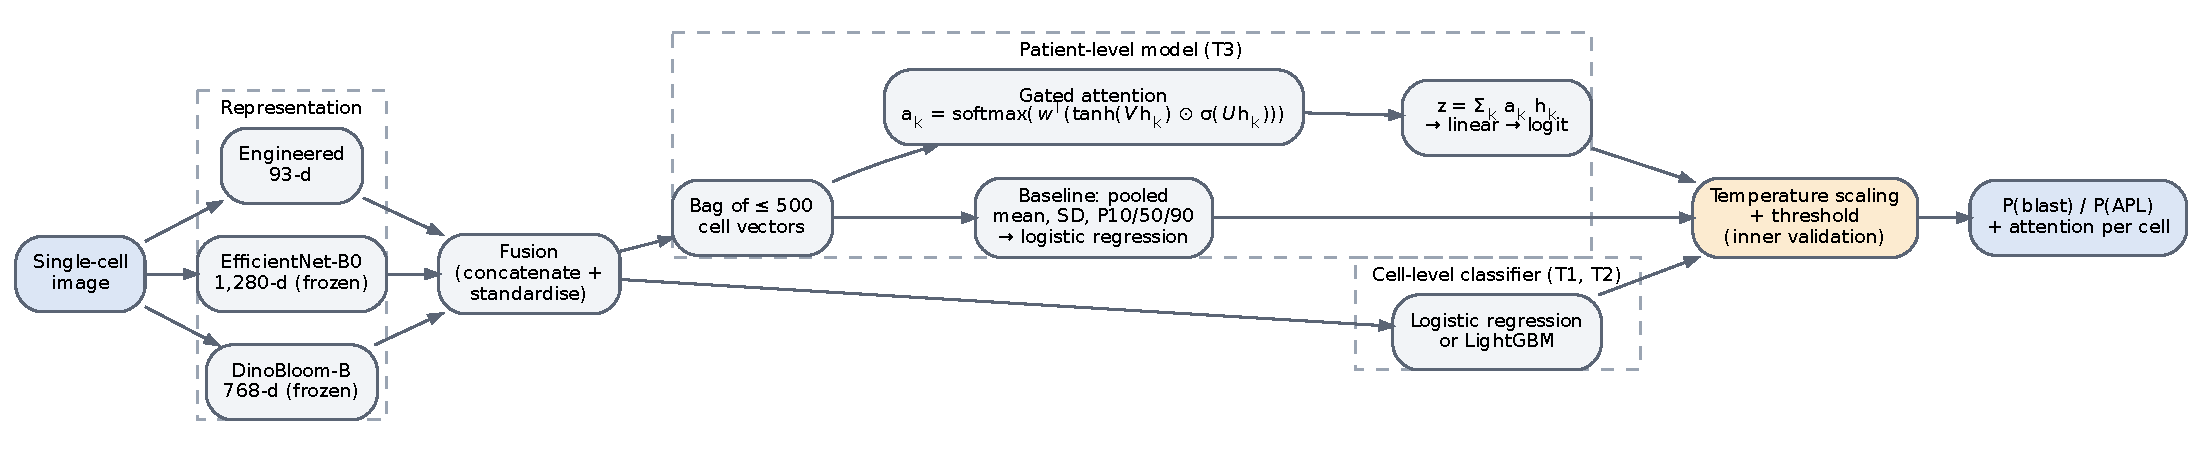
\includegraphics[width=\textwidth]{fig_model.pdf}
\caption{Model overview. Each cell is described by engineered features, a frozen CNN embedding (optionally reduced by PCA), their fusion, or a partially fine-tuned CNN with average or attention pooling. Cell-level classifiers serve T1, T2 and T4. For patients and subjects (T3, T5), the cells are combined by pooled statistics, by gated attention MIL or by averaging fine-tuned cell probabilities, and the three can be combined in a pre-specified ensemble. The decision threshold is set on development data for a recall of at least 0.95.}
\label{fig:model}
\end{figure*}

For patient diagnosis (T3) each patient is represented by up to 500 randomly sampled cells. The pooled baseline summarizes every feature by its mean, standard deviation and 10th, 50th and 90th percentiles and applies LR. The gated attention MIL model \cite{ilse2018abmil} maps each cell to $\mathbf{h}_k=\mathrm{ReLU}(\mathbf{W}\mathbf{x}_k)$ with 128 units, weights the cells by
\begin{equation}
a_k=\frac{\exp\{\mathbf{w}^{\top}(\tanh(\mathbf{V}\mathbf{h}_k)\odot\sigma(\mathbf{U}\mathbf{h}_k))\}}{\sum_{j}\exp\{\mathbf{w}^{\top}(\tanh(\mathbf{V}\mathbf{h}_j)\odot\sigma(\mathbf{U}\mathbf{h}_j))\}},
\end{equation}
and classifies the weighted average $\mathbf{z}=\sum_k a_k\mathbf{h}_k$. Because the weights sum to one, the model does not depend on how many cells a patient has. It is trained for 40 epochs with AdamW (learning rate $2\times10^{-4}$, weight decay $10^{-3}$), class-weighted cross-entropy and random removal of 20\% of cells as augmentation.

\subsection{Final Pipelines and Pre-Specification}
\label{sec:final}
Before the final analysis we fixed one primary pipeline and one secondary pipeline and committed the specification, with time stamp, to the code repository. The primary pipeline (Fig.~\ref{fig:pipelines}a) normalizes stains when the shift test is positive, classifies every cell with the fine-tuned CNN, and combines three patient-level scores---the mean fine-tuned cell probability, engineered features with pooled statistics, and engineered features with attention MIL---in an ensemble that averages their percentile scores; the decision threshold is set on development data for a recall of at least 0.95. The secondary pipeline (Fig.~\ref{fig:pipelines}b) was declared as a low-complexity option: stain normalization, the frozen CNN, PCA with 64 components, pooled statistics and logistic regression. It was chosen to reduce storage, model size and training time, not to improve accuracy, and we report its cost in performance alongside its savings. The preprocessing comparison and a pilot of the secondary pipeline used a subset that included the APL-AML Validation patients; the choice of the primary pipeline did not depend on those numbers, and C-NMC and the pooled analysis provide confirmation outside that cohort.

\begin{figure*}[!t]
\centering
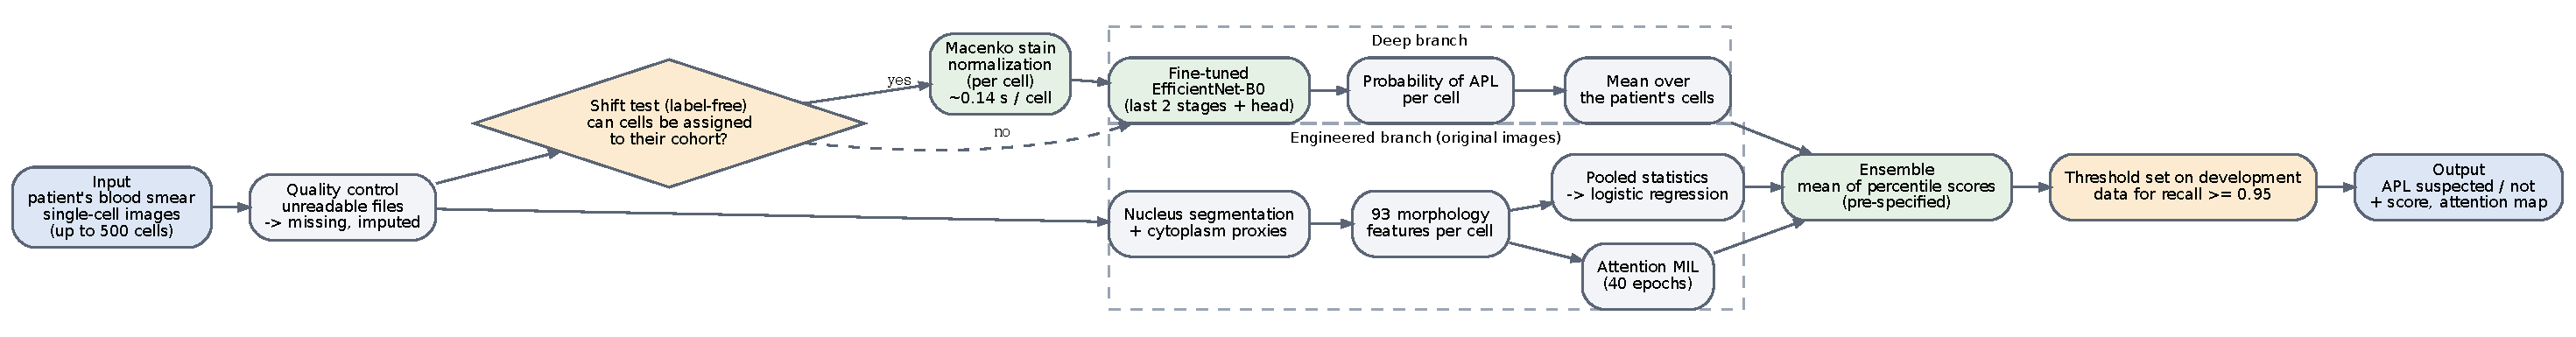
\includegraphics[width=\textwidth]{fig_pipeline_primary.pdf}\\[2pt]
{\footnotesize (a) Primary pipeline}\\[6pt]
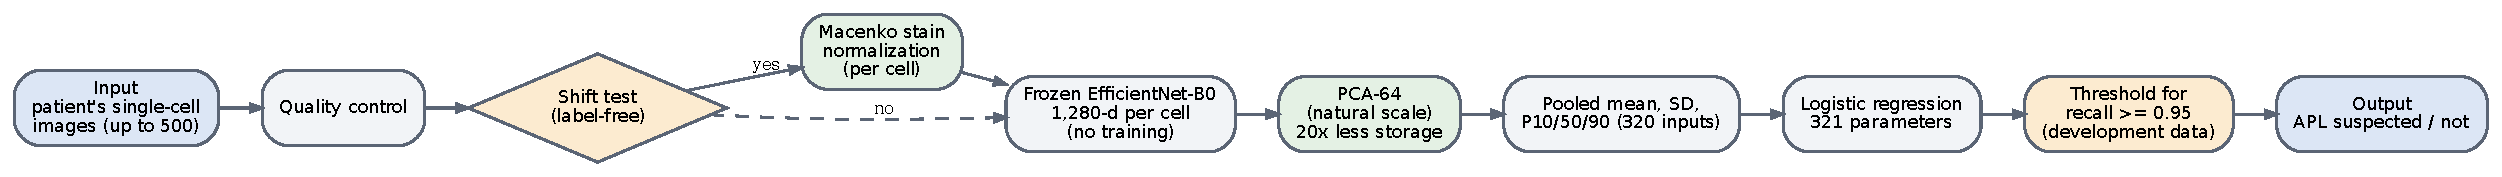
\includegraphics[width=0.86\textwidth]{fig_pipeline_secondary.pdf}\\[2pt]
{\footnotesize (b) Secondary, low-complexity pipeline}
\caption{End-to-end pipelines from the single-cell images of a patient to the decision. Orange: steps fixed on development data (shift test, threshold). Green: components retained because they improved external performance (stain normalization, fine-tuning, ensemble) or reduced complexity (PCA).}
\label{fig:pipelines}
\end{figure*}

\subsection{Evaluation Protocol and Metrics}
Every model was evaluated in three ways (Fig.~\ref{S-fig:splits}): 5-fold CV on the Discovery cohort with image-level folds, as is common in the literature; 5-fold CV with patient-grouped folds, in which no patient appears in two folds; and a single external test on the Validation cohort. Within each training fold, a further 80/20 split of the same kind was used to fit a calibration temperature \cite{guo2017calibration}. For the external test of T3, the prediction for each Validation patient is the average of all fold models over three seeds, and the decision threshold is chosen on the out-of-fold Discovery predictions of the same models.



Since missing an APL patient can delay life-saving treatment, whereas a false alarm leads only to a confirmatory genetic test, we fixed every decision threshold in advance to reach a sensitivity of at least 0.95 on development data. At that operating point we report sensitivity (recall) together with the number of missed positives, specificity, F1 score, negative predictive value (NPV) and accuracy. AUROC is reported as a threshold-free summary, and calibration as the expected calibration error (ECE, 15 bins). Confidence intervals (95\%) come from bootstrap resampling of patients \cite{efron1986bootstrap}, because cells from the same patient are correlated, and differences between two models are tested with a paired patient-level bootstrap. When a table reports several comparisons against the same reference, $p$-values are also given after Holm correction \cite{holm1979}. C-NMC was analyzed with exactly the same protocol, with folds 0--1 in the role of Discovery and fold 2 in the role of Validation.

Three further analyses address questions that the external tests alone cannot answer. First, because 24 external patients give wide confidence intervals, we repeated the main patient-level comparisons with three repeats of 5-fold patient-level CV over all 106 APL-AML patients, stratified by diagnosis and cohort; thresholds were chosen by an inner CV inside each training fold. This analysis has more statistical power but gives up the temporal separation, so it complements rather than replaces the external test. Second, to see whether a new laboratory could restore the intended operating point, we simulated local recalibration: $k$ confirmed local patients ($k/2$ APL, $k/2$ AML, $k=2,\dots,8$) were drawn from the Validation cohort, the threshold was lowered if needed to just below the lowest score of the local APL cases, and the remaining $24-k$ patients were scored, over 2,000 random draws. Third, decision-curve analysis \cite{vickers2006dca} estimated the net benefit of acting on the model's output at an APL prevalence of 10\%, closer to that among patients with suspected acute leukemia than the 50\% of the Validation cohort; predicted probabilities were mapped to risks by logistic recalibration on Discovery and shifted to the target prevalence.

\subsection{Implementation Details}
All experiments ran on a CPU-only workstation without a GPU (Table~\ref{S-tab:env}). Feature extraction dominates the cost; once features are stored, each cell-level configuration trains and evaluates in under a minute and each patient-level configuration in about a minute. Table~\ref{S-tab:hparams} lists every setting of every component. All of them were fixed in advance or taken from library defaults; the Validation cohort was scored only after the configuration had been frozen, and no setting was changed afterwards. The attention MIL model is trained for a fixed 40 epochs without early stopping, so no held-out data is consumed for model selection; its training curves are examined in Section~\ref{sec:training}.




%======================================================================
\section{Results}
\subsection{Exploratory Analysis of Both Datasets}
\label{sec:eda}
Both datasets are imbalanced, and in different ways (Tables~\ref{tab:dataset} and \ref{tab:dataset_cnmc}). APL makes up 27\% of Discovery and 50\% of Validation patients; ALL makes up 71\% of C-NMC development and 55\% of external subjects, and about two thirds of the cells in both C-NMC sets. We therefore used class-balanced weights in every classifier, did not resample cells, set thresholds for the minority (positive) class, and report metrics that do not depend on prevalence or that show the errors directly---recall, specificity, missed cases, F1 score and AUROC---rather than accuracy alone.

Fig.~\ref{fig:eda} summarizes the exploratory analysis of the engineered features. Every feature group shifted between the two cohorts, and stain and color features shifted most (median standardized mean difference 0.34, Fig.~\ref{fig:eda}a). The shift was large enough to recognize the cohort: among AML patients only, a classifier separated Validation from Discovery cells with an AUROC of 0.75 using stain and color features, compared with 0.59 for shape and texture features and 0.58 for EfficientNet-B0 embeddings (Fig.~\ref{fig:eda}b). Thirty-seven feature pairs were almost redundant ($|r|>0.9$). The diagnostic signal of individual features was only partly reproducible: patient-level AUROCs in the two cohorts correlated with $r=0.38$, and 11 of 93 features separated APL from AML in the same direction in both cohorts (Fig.~\ref{fig:eda}d). These observations motivated the preprocessing and feature-engineering experiments below.

C-NMC looked very different (Fig.~\ref{fig:eda_cnmc}). Feature shifts between the development and external sets were small (median standardized difference 0.04--0.16 per group, 0.14 for stain and color), and a classifier could not tell external from development cells of normal subjects (AUROC 0.44--0.52, chance level, for every representation). The diagnostic signal of single features was more reproducible ($r=0.48$; 18 of 93 features consistent in both sets), and 57 feature pairs were nearly redundant. In short, APL-AML has a measurable acquisition shift and C-NMC does not, a difference that explains several results below.

\begin{table}[!t]
\centering
\caption{Composition of the C-NMC 2019 data used here (official training folds).}
\label{tab:dataset_cnmc}
\resizebox{\columnwidth}{!}{%
\begin{tabular}{llrrr}
\toprule
Set & Class & Subjects & Cells & Cells per subject, median (range) \\
\midrule
Development & Normal B cells & 12 & 2,293 & 140 (18--405) \\
Development & ALL & 30 & 4,815 & 112 (9--757) \\
External & Normal B cells & 14 & 1,096 & 41 (9--327) \\
External & ALL & 17 & 2,457 & 161 (14--278) \\
\midrule
Total & & 73 & 10,661 & \\
\bottomrule
\end{tabular}}
\end{table}

\begin{figure*}[!t]
\centering
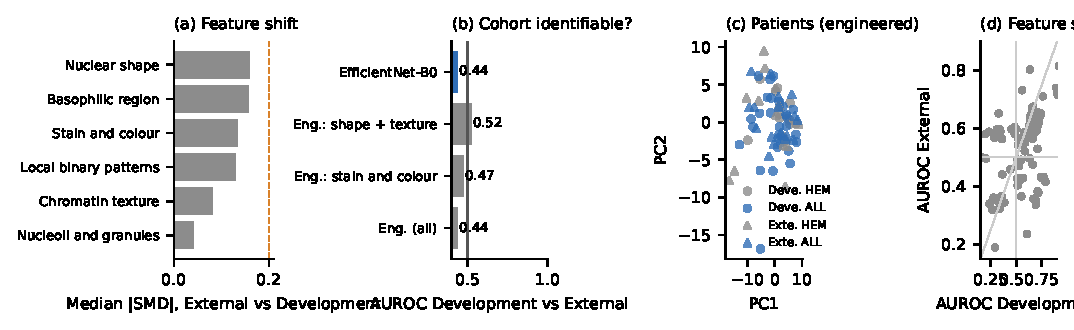
\includegraphics[width=0.9\textwidth]{fig_eda_cnmc.pdf}
\caption{Exploratory analysis of C-NMC (development: folds 0--1; external: fold 2), in the same layout as Fig.~\ref{fig:eda}. (a) Shift of feature groups. (b) Cohort identifiability; values near 0.5 mean that external and development cells cannot be told apart. (c) Subjects on the first two principal components of their mean engineered features. (d) Subject-level AUROC of each feature in the two sets.}
\label{fig:eda_cnmc}
\end{figure*}

\begin{figure*}[!t]
\centering
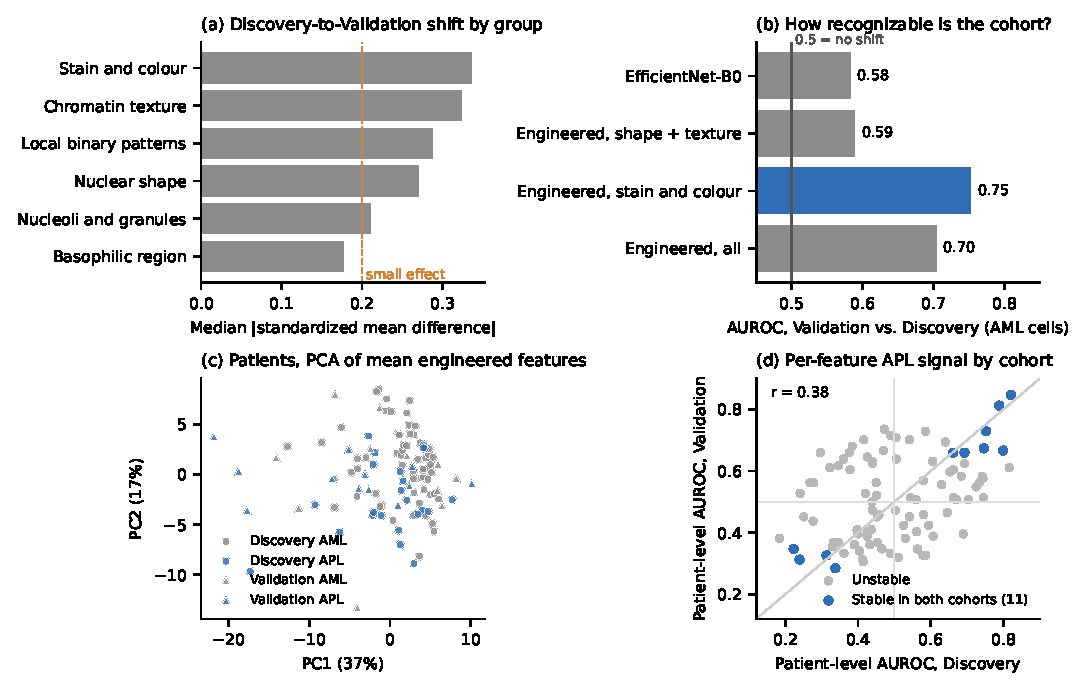
\includegraphics[width=0.9\textwidth]{fig_eda.pdf}
\caption{Exploratory analysis. (a) Shift of engineered feature groups from Discovery to Validation. (b) AUROC of a classifier that tries to tell the two cohorts apart from AML cells; 0.5 means no detectable shift. (c) Patients projected on the first two principal components of their mean engineered features. (d) Patient-level AUROC of each feature for APL vs.\ AML in the two cohorts; blue points separate the classes consistently.}
\label{fig:eda}
\end{figure*}

\subsection{Effect of the Evaluation Protocol}
Table~\ref{tab:leakage} and Fig.~\ref{fig:leakage} compare the three protocols. When each cell carried its patient's diagnosis (T1), image-level CV reported AUROCs of 0.938--0.987. Grouping folds by patient lowered them to 0.867--0.901, and the external cohort to 0.658--0.734, so image-level CV overstated external performance by 0.25 to 0.32. When the label described the cell itself (T2), the three protocols nearly agreed and the overstatement was 0.013--0.036. The models themselves changed little: a classifier trained under the leaky protocol scored about the same on the external cohort as one trained under the grouped protocol. What changed was the number reported. The same pattern appeared on C-NMC (Table~\ref{tab:cnmc}a), where every cell also carries its subject's diagnosis: image-level CV reported 0.912--0.939, subject-grouped CV 0.834--0.864 and the external fold 0.775--0.840, an overstatement of 0.09--0.14. The inflation was smaller than for T1, consistent with C-NMC labels being partly a property of the cell, since the ALL cells were selected as malignant lymphoblasts. Table~\ref{tab:reported} shows what this means in the terms most studies report: evaluated with image-level CV at the usual 0.5 threshold, the same models reached accuracies of 0.88--0.95, whereas on new patients accuracy was 0.69--0.73 for diagnosis from single APL-AML cells, 0.87--0.90 for blasts and 0.82--0.83 on C-NMC. For diagnosis from single cells, the default threshold recovered only 25--37\% of the cells of new APL patients, a failure that the leaky protocol hides completely.

\begin{table*}[!t]
\centering
\caption{The same models evaluated the way many studies report them (image-level 5-fold CV, accuracy at a 0.5 threshold) and on patients they have never seen (external set). Mean over seeds.}
\label{tab:reported}
\setlength{\tabcolsep}{4pt}
\resizebox{\textwidth}{!}{%
\begin{tabular}{llccccccc}
\toprule
 & & \multicolumn{3}{c}{Image-level CV (leaky)} & \multicolumn{4}{c}{External set (new patients)} \\
\cmidrule(lr){3-5}\cmidrule(lr){6-9}
Task & Model & Accuracy & AUROC & F1 & Accuracy & AUROC & Recall & F1 \\
\midrule
T1 APL-AML, diagnosis on cells & Engineered + LightGBM & 0.950 & 0.987 & 0.942 & 0.691 & 0.669 & 0.245 & 0.342 \\
 & Fusion + LR & 0.942 & 0.985 & 0.933 & 0.715 & 0.734 & 0.370 & 0.466 \\
 & Fine-tuned EfficientNet-B0 & -- & -- & -- & 0.732 & 0.773 & 0.340 & 0.464 \\
\midrule
T2 APL-AML, blast detection & Engineered + LightGBM & 0.928 & 0.978 & 0.875 & 0.898 & 0.957 & 0.895 & 0.786 \\
 & Fusion + LR & 0.911 & 0.964 & 0.845 & 0.866 & 0.932 & 0.850 & 0.725 \\
 & Fine-tuned EfficientNet-B0 & -- & -- & -- & 0.904 & 0.960 & 0.883 & 0.792 \\
\midrule
T4 C-NMC, cells & Engineered + LR & 0.877 & 0.933 & 0.907 & 0.827 & 0.840 & 0.896 & 0.877 \\
 & Fusion + LR & 0.894 & 0.939 & 0.921 & 0.816 & 0.817 & 0.895 & 0.871 \\
 & Fine-tuned EfficientNet-B0 & -- & -- & -- & 0.825 & 0.841 & 0.946 & 0.882 \\
\bottomrule
\end{tabular}}
\end{table*}

\begin{table*}[!t]
\centering
\caption{Effect of the evaluation protocol at cell level (mean of three seeds). AUROC under image-level CV, patient-grouped CV and on the external Validation cohort; threshold metrics on the external cohort at the operating point fixed on Discovery (target sensitivity 0.95). Inflation = image-level CV AUROC minus external AUROC.}
\label{tab:leakage}
\setlength{\tabcolsep}{3.5pt}
\begin{tabular}{llccccccccc}
\toprule
 & & \multicolumn{3}{c}{AUROC} & \multicolumn{5}{c}{External cohort, fixed operating point} & \\
\cmidrule(lr){3-5}\cmidrule(lr){6-10}
Task & Model & Image CV & Grouped CV & External [95\% CI] & Recall & Spec. & F1 & NPV & Acc. & Inflation \\
\midrule
T1 Diagnosis on cells & Engineered + LightGBM & 0.987 & 0.896 & 0.669 [0.495, 0.811] & 0.69 & 0.55 & 0.54 & 0.78 & 0.60 & +0.318 \\
 & Engineered + LR & 0.938 & 0.895 & 0.658 [0.478, 0.798] & 0.73 & 0.46 & 0.52 & 0.77 & 0.55 & +0.280 \\
 & EfficientNet-B0 + LR & 0.975 & 0.867 & 0.694 [0.556, 0.811] & 0.81 & 0.43 & 0.56 & 0.81 & 0.56 & +0.281 \\
 & Fusion + LR & 0.985 & 0.901 & \textbf{0.734 [0.595, 0.848]} & 0.78 & 0.54 & 0.59 & 0.83 & 0.62 & +0.250 \\
\midrule
T2 Blast detection & Engineered + LightGBM & 0.978 & 0.954 & \textbf{0.957 [0.931, 0.977]} & 0.99 & 0.62 & 0.58 & 1.00 & 0.70 & +0.021 \\
 & Engineered + LR & 0.965 & 0.951 & 0.951 [0.922, 0.972] & 0.98 & 0.70 & 0.63 & 0.99 & 0.76 & +0.013 \\
 & EfficientNet-B0 + LR & 0.956 & 0.927 & 0.920 [0.874, 0.956] & 0.96 & 0.64 & 0.58 & 0.98 & 0.70 & +0.036 \\
 & Fusion + LR & 0.964 & 0.940 & 0.932 [0.894, 0.961] & 0.96 & 0.68 & 0.61 & 0.99 & 0.74 & +0.033 \\
\bottomrule
\end{tabular}
\end{table*}

\begin{figure*}[!t]
\centering
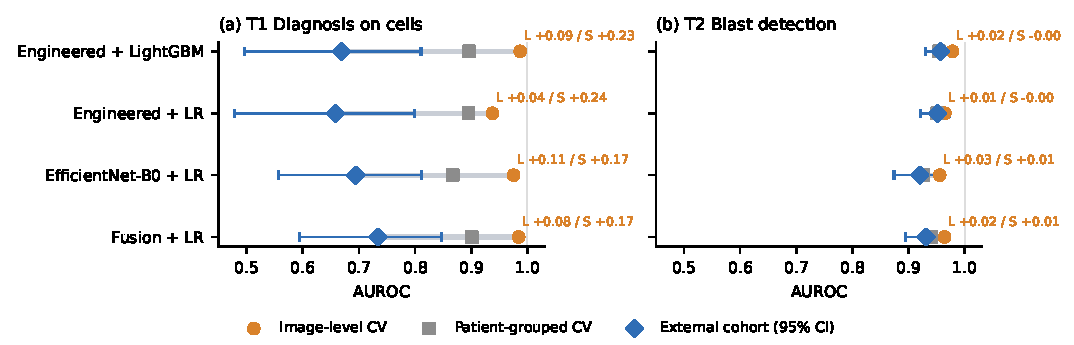
\includegraphics[width=\textwidth]{fig_leakage.pdf}
\caption{AUROC under the three protocols (mean of three seeds). Orange numbers give the inflation of image-level CV over the external cohort. (a) Cells labeled with the patient's diagnosis. (b) Cells labeled with their own type.}
\label{fig:leakage}
\end{figure*}

\subsection{Preprocessing: Choosing a Stain Normalization}
\label{sec:preproc}
Table~\ref{tab:preproc} compares the preprocessing options on a fixed subset of up to 60 cells per patient, with the same folds and classifiers for every option. Edge sharpening raised development performance slightly (cells 0.873 to 0.887) but lowered it on new patients (cells 0.661 to 0.631; patients 0.667 to 0.639), so it widened the gap between development and external results; sharpening amplifies fine, acquisition-specific detail such as compression artifacts. Reinhard normalization removed most of the measurable cohort shift (0.575 to 0.524) and reduced the spread across folds, but external performance at cell level fell (0.644). Macenko normalization reduced the shift (0.543) and was the only option that raised external performance at both levels (cells 0.690, patients 0.694), narrowing the gap between development and external AUROC from 0.21 to 0.16 for cells and from 0.29 to 0.25 for patients. It therefore met the rule fixed in advance and was selected. Estimating stain vectors once per patient instead of once per cell was about 70 times faster but lowered patient-level development CV by 0.017 and failed the pre-specified rule, so normalization is done per cell. On C-NMC, where no shift was detectable, Macenko normalization lowered external AUROC slightly (cells 0.746 to 0.729, subjects 0.882 to 0.857), which supports applying it only when a shift is present. All of these differences are small compared with the uncertainty of 24 external patients; the clearest benefit appeared at the operating point of the frozen-CNN models on the full data (Section~\ref{sec:finalres}).

\begin{table*}[!t]
\centering
\caption{Preprocessing before feature extraction (frozen EfficientNet-B0, up to 60 cells per patient, same folds and classifiers for every variant). Cohort shift: AUROC for assigning control-class cells to their cohort (0.5 = no detectable shift). Gap: development CV minus external AUROC. The rule fixed in advance selected the method that reduced the shift without lowering external performance. C-NMC, which showed no shift, is given for comparison.}
\label{tab:preproc}
\setlength{\tabcolsep}{3.2pt}
\resizebox{\textwidth}{!}{%
\begin{tabular}{lccccccc}
\toprule
 & & \multicolumn{3}{c}{Cells (T1)} & \multicolumn{3}{c}{Patients (T3)} \\
\cmidrule(lr){3-5}\cmidrule(lr){6-8}
Preprocessing & Cohort shift & Dev.\ CV (SD; worst fold) & External & Gap & Dev.\ CV (SD; worst fold) & External & Gap \\
\midrule
\multicolumn{8}{l}{\emph{APL-AML (6,360 cells, 106 patients)}} \\
None & 0.575 & 0.873 (0.036; 0.818) & 0.661 & 0.212 & 0.956 (0.047; 0.875) & 0.667 & 0.289 \\
Edge sharpening (unsharp mask) & 0.561 & 0.887 (0.030; 0.834) & 0.631 & 0.256 & 0.963 (0.050; 0.875) & 0.639 & 0.324 \\
Reinhard colour normalization & 0.524 & 0.873 (0.026; 0.836) & 0.644 & 0.228 & 0.972 (0.039; 0.896) & 0.681 & 0.291 \\
\textbf{Macenko stain normalization (selected)} & 0.543 & 0.850 (0.037; 0.785) & 0.690 & 0.160 & 0.942 (0.052; 0.875) & 0.694 & 0.247 \\
Macenko, stain vectors per patient & 0.554 & 0.859 (0.048; 0.775) & 0.615 & 0.244 & 0.925 (0.070; 0.833) & 0.611 & 0.314 \\
\midrule
\multicolumn{8}{l}{\emph{C-NMC (3,773 cells, 73 subjects; no shift detected)}} \\
None & 0.549 & 0.832 (0.050; 0.753) & 0.746 & 0.086 & 0.889 (0.222; 0.444) & 0.882 & 0.007 \\
Macenko stain normalization & 0.560 & 0.818 (0.058; 0.708) & 0.729 & 0.088 & 0.861 (0.238; 0.389) & 0.857 & 0.004 \\
\bottomrule
\end{tabular}}
\end{table*}

\subsection{Engineered, Frozen and Fine-Tuned Deep Features at Cell Level}
For blast detection on new patients, engineered features with LightGBM reached an AUROC of 0.957 (95\% CI 0.931--0.977) and detected 99\% of blasts at a specificity of 0.62, whereas EfficientNet-B0 embeddings reached 0.920. The paired difference was $+0.034$ (0.008--0.065, $p=0.002$), and fusing both representations also improved on the embeddings alone ($+0.012$, 0.003--0.024). For diagnosis-on-cells (T1), fusion gave the highest external AUROC among the frozen representations (0.734), although its advantage was not significant. On C-NMC, engineered features again outperformed the frozen embedding on the external fold (0.840 vs.\ 0.775, Table~\ref{tab:cnmc}a).

Fine-tuning changed the picture for T1 (Table~\ref{tab:finetune}). Adapting the last stages of EfficientNet-B0 raised external AUROC to 0.773 (95\% CI 0.612--0.890), the highest of all cell-level models, against 0.694 for the same network used as a frozen feature extractor. The fine-tuned model did not escape the operating-point problem, however: the threshold chosen on Discovery for a sensitivity of 0.95 flagged nearly every Validation cell (recall 0.996, specificity 0.17). For blast detection, fine-tuning reached an external AUROC of 0.960 (0.928--0.981), similar to the engineered features (0.957), but with a much better operating point: at a recall of 0.95 its specificity was 0.84 instead of 0.62, and its F1 score 0.74 instead of 0.58. On C-NMC cells, fine-tuning raised external AUROC from 0.775 (frozen) to 0.841, level with engineered features (0.840), and reached a recall of 0.99.

\begin{table*}[!t]
\centering
\caption{Engineered, frozen and fine-tuned features at cell level on both datasets. The fine-tuned model adapts the last two stages of EfficientNet-B0 (Table~\ref{S-tab:hparams}; one seed); the other models are averaged over three seeds. Inflation: image-level CV AUROC minus external AUROC. Recall, specificity and F1 on the external set at the operating point fixed on development data. Best external AUROC per task in bold.}
\label{tab:finetune}
\setlength{\tabcolsep}{3.5pt}
\resizebox{\textwidth}{!}{%
\begin{tabular}{llccccccc}
\toprule
Task & Model & Image CV & Grouped CV & External [95\% CI] & Inflation & Recall & Spec. & F1 \\
\midrule
T1 APL-AML, diagnosis on cells & Engineered + LightGBM & 0.987 & 0.896 & 0.669 [0.495, 0.811] & +0.318 & 0.69 & 0.55 & 0.54 \\
 & Engineered + LR & 0.938 & 0.895 & 0.658 [0.478, 0.798] & +0.280 & 0.73 & 0.46 & 0.52 \\
 & EfficientNet-B0 + LR & 0.975 & 0.867 & 0.694 [0.556, 0.811] & +0.281 & 0.81 & 0.43 & 0.56 \\
 & Fusion + LR & 0.985 & 0.901 & 0.734 [0.595, 0.848] & +0.250 & 0.78 & 0.54 & 0.59 \\
 & Fine-tuned EfficientNet-B0 & -- & 0.875 & \textbf{0.773 [0.612, 0.890]} & -- & 1.00 & 0.17 & 0.55 \\
\midrule
T2 APL-AML, blast detection & Engineered + LightGBM & 0.978 & 0.954 & 0.957 [0.931, 0.977] & +0.021 & 0.99 & 0.62 & 0.58 \\
 & Engineered + LR & 0.965 & 0.951 & 0.951 [0.922, 0.972] & +0.013 & 0.98 & 0.70 & 0.63 \\
 & EfficientNet-B0 + LR & 0.956 & 0.926 & 0.920 [0.874, 0.956] & +0.036 & 0.96 & 0.64 & 0.58 \\
 & Fusion + LR & 0.964 & 0.940 & 0.931 [0.894, 0.961] & +0.033 & 0.96 & 0.68 & 0.61 \\
 & Fine-tuned EfficientNet-B0 & -- & 0.968 & \textbf{0.960 [0.928, 0.981]} & -- & 0.95 & 0.83 & 0.74 \\
\midrule
T4 C-NMC, cells & Engineered + LR & 0.933 & 0.864 & 0.840 [0.730, 0.902] & +0.093 & 0.95 & 0.58 & 0.89 \\
 & EfficientNet-B0 + LR & 0.912 & 0.834 & 0.775 [0.640, 0.859] & +0.137 & 0.96 & 0.43 & 0.87 \\
 & Fusion + LR & 0.939 & 0.864 & 0.817 [0.692, 0.891] & +0.122 & 0.95 & 0.54 & 0.88 \\
 & Fine-tuned EfficientNet-B0 & -- & 0.853 & \textbf{0.841 [0.715, 0.917]} & -- & 0.99 & 0.42 & 0.88 \\
\bottomrule
\end{tabular}}
\end{table*}

\subsection{Feature Engineering}
Table~\ref{S-tab:fe} reports the feature-engineering experiments for patient-level APL detection. These experiments used our first PCA implementation, in which each principal component was standardized before the classifier (Section~\ref{sec:pca} explains why this matters). On the Validation cohort, dimensionality reduction had the largest effect. The configuration chosen by the rule fixed in advance---the highest Discovery CV AUROC---was PCA with 64 components, which raised external AUROC from 0.743 to 0.819; 32 components gave the highest external value (0.833), and 16 components the best operating point, detecting 11 of 12 APL patients at a specificity of 0.67. None of these gains was statistically significant, and after Holm correction no feature-engineering step differed significantly from its unreduced reference. Section~\ref{sec:pca} shows that this gain did not reproduce with correctly scaled components, in pooled CV or on C-NMC. Removing redundant engineered features changed little. Normalizing stain features within each slide and L1 selection both lowered external AUROC, to 0.58 and 0.59: the color of a patient's cells carries diagnostic information---APL promyelocytes are heavily granulated---that slide-wise normalization removes, and L1 selection with 82 patients chose unstable features. A ``digital differential'' built from the predicted proportions of eight cell classes reached 0.785 and detected all 12 APL patients, at a specificity of 0.33. 


\subsection{Dimensionality Reduction: Before and After PCA}
\label{sec:pca}
Table~\ref{tab:pcaimpact} summarizes the impact of PCA on the pooled patient model built from EfficientNet-B0 embeddings, and Table~\ref{S-tab:pca} and Fig.~\ref{fig:pca} give the full sweep over the number of components on both datasets. Without reduction, each patient is described by 6,400 values (five statistics of 1,280 dimensions), about 100 for every APL-AML training patient.

\emph{Before and after on APL-AML.} PCA improved how well patients were ranked but not the decisions made at the clinical operating point. External AUROC rose from 0.708 without PCA to 0.785 with 32 and 0.792 with 64 components, and stayed at 0.778 up to 256 components; the pre-declared rule (highest Discovery CV) selected 256 components. At the threshold fixed on Discovery, however, the unreduced model detected 8 of 12 APL patients and the reduced models 6 of 12, at specificities of 0.67 and 0.75; accuracy fell from 0.67 to 0.63 and F1 from 0.67 to 0.57. Fewer than 16 components discarded diagnostic information (8 components: AUROC 0.646).

\emph{Before and after on C-NMC.} Here PCA cost a little on every metric. External AUROC was 0.908 without PCA and rose steadily with the number of components (8: 0.803; 32: 0.840; 64: 0.853; 256: 0.870) without reaching the unreduced value, and the pre-declared rule selected no reduction. At the operating point, the unreduced model detected all 17 ALL subjects with an accuracy of 0.84 and F1 of 0.87; with 32--64 components, 16 of 17 were detected, accuracy was 0.71--0.74 and F1 0.78--0.80.

\emph{With more statistical power.} In pooled CV over all 106 APL-AML patients, 32 and 64 components ranked patients as well as the unreduced embedding ($\Delta$AUROC $+0.000$ and $+0.006$; Table~\ref{S-tab:pooled}), and 16 components were significantly worse ($-0.057$). The APL-AML gain on the 24-patient temporal test therefore did not reflect a general advantage.

\emph{A pitfall: whitening.} In our first analysis the pooled component scores were standardized one by one before the classifier, as is common practice. This whitens the representation: low-variance components, which mostly carry noise, are inflated to the same scale as the leading ones and weighted equally by the L2 penalty. With whitening, external AUROC behaved erratically---on C-NMC it fell from 0.849 at 8 to 0.655 at 256 components, far below the unreduced 0.908, while development CV rose to 0.99 (Table~\ref{S-tab:pca}, column Std.; dashed lines in Fig.~\ref{fig:pca})---and on APL-AML it produced the largest apparent gain (0.833 with 32 components). Keeping the components at their natural scale removed both effects. The rising development CV together with falling external AUROC is the signature of a classifier fitting noise directions, and it is a warning that dimensionality and scaling choices should not be tuned on development CV.

\emph{Why PCA gives no consistent edge.} PCA keeps the directions of largest variance, not those that separate the classes. The diagnostics in Fig.~\ref{fig:pca}c show that the external cell-level disease signal increased steadily with the number of components on both datasets, so the discarded low-variance components still carry diagnostic information---especially on C-NMC, where malignant and normal B cells differ subtly. Nor did PCA remove acquisition-specific information: a classifier separating external from development cells of the control class performed about equally on every representation (APL-AML 0.57--0.64; C-NMC 0.45--0.56). What PCA does is shrink the patient-level model, and on the shifted APL-AML cohort this improved ranking, presumably by discarding some development-specific variation together with some signal; on C-NMC, without such a shift, the lost signal dominated. Unsupervised dimensionality reduction is therefore a reasonable way to make patient-level models smaller, but not a reliable way to make them more accurate.

\begin{table}[!t]
\centering
\caption{Impact of PCA on patient/subject-level detection (external sets). Before: unreduced 1,280-dimensional embedding. After: PCA fitted on development cells, scores kept at their natural scale. Rule: number of components with the highest development CV AUROC (pre-declared). Threshold metrics at the operating point fixed on development data.}
\label{tab:pcaimpact}
\setlength{\tabcolsep}{2.4pt}
\resizebox{\columnwidth}{!}{%
\begin{tabular}{llccccccc}
\toprule
Dataset & Representation & AUROC & $\Delta$AUROC & Acc. & Recall (missed) & Spec. & F1 & NPV \\
\midrule
APL-AML & Before: no PCA & 0.708 & -- & 0.67 & 0.67 (4/12) & 0.67 & 0.67 & 0.67 \\
 & After: PCA-32 & 0.785 & +0.076 & 0.62 & 0.50 (6/12) & 0.75 & 0.57 & 0.60 \\
 & After: PCA-64 & 0.792 & +0.083 & 0.62 & 0.50 (6/12) & 0.75 & 0.57 & 0.60 \\
 & After: PCA-256 (rule) & 0.778 & +0.069 & 0.62 & 0.50 (6/12) & 0.75 & 0.57 & 0.60 \\
\midrule
C-NMC & Before: no PCA & 0.908 & -- & 0.84 & 1.00 (0/17) & 0.64 & 0.87 & 1.00 \\
 & After: PCA-32 & 0.840 & -0.067 & 0.71 & 0.94 (1/17) & 0.43 & 0.78 & 0.86 \\
 & After: PCA-64 & 0.853 & -0.055 & 0.74 & 0.94 (1/17) & 0.50 & 0.80 & 0.88 \\
 & No PCA (rule) & 0.908 & -- & 0.84 & 1.00 (0/17) & 0.64 & 0.87 & 1.00 \\
\bottomrule
\end{tabular}}
\end{table}


\begin{figure*}[!t]
\centering
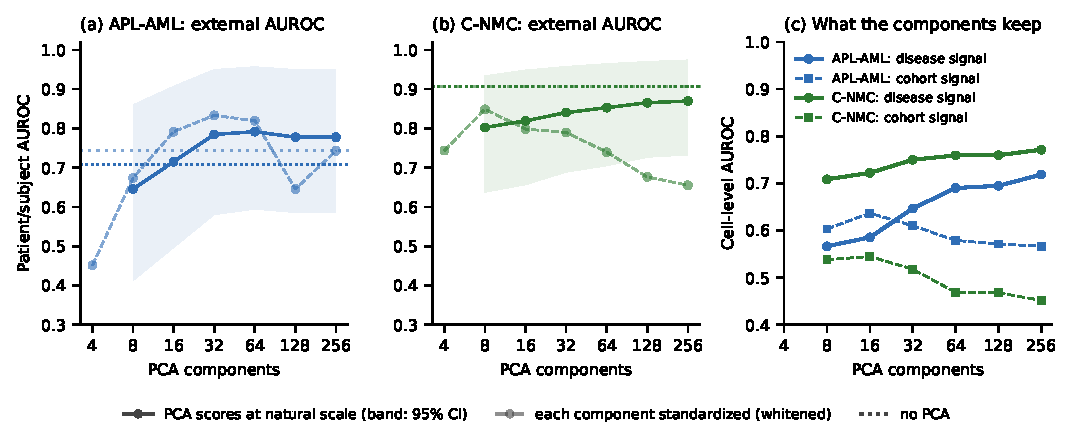
\includegraphics[width=\textwidth]{fig_pca_two.pdf}
\caption{PCA of EfficientNet-B0 embeddings, pooled patient/subject model. (a) APL-AML and (b) C-NMC: external AUROC versus the number of components with the component scores kept at their natural scale (solid; band: 95\% CI) and with each component standardized, i.e., whitened (dashed); horizontal lines: no PCA under the same scaling. (c) What the components keep: external cell-level disease signal (circles) and cohort signal, i.e., AUROC for telling external from development cells of the control class (squares; 0.5 = none).}
\label{fig:pca}
\end{figure*}

\subsection{Training Settings: Epochs, Early Stopping and Pooling}
\label{sec:training}
Because the number of training epochs can shape both performance and calibration, we tested a data-driven alternative to the fixed 40 epochs of attention MIL: inside every training fold, a nested 3-fold patient-level CV chose the epoch with the lowest mean validation loss, and the model was retrained on the whole fold for that many epochs. Table~\ref{S-tab:epochs} shows that this did not help. External AUROC changed by less than 0.01 on APL-AML (e.g., 0.812 vs.\ 0.819 for engineered features) and fell by 0.02--0.06 on C-NMC; F1 score and calibration did not improve. The chosen number of epochs varied widely for the same model, from 1 to 40, because each inner model was trained on about 35 and validated on about 17 patients, and early stopping made results less consistent across seeds (development CV 0.770--0.852 vs.\ 0.824--0.830). We therefore kept the fixed schedule. The models with CNN features tended to stop after 4--5 epochs, in line with the learning curves below, which show their validation loss bottoming out early. The fine-tuned CNN already selects its best epoch on inner validation patients within a short, decaying learning-rate schedule (6 epochs), so it needs no further stopping rule.

We also replaced the average pooling of the fine-tuned CNN with gated attention pooling over the $7\times7$ spatial positions. On the first three of five development folds, attention changed AUROC by $-0.020$, $+0.014$ and $+0.005$ (mean $0.000$), and we did not pursue it further.


\emph{Learning curves.}
Fig.~\ref{S-fig:training} shows how the trainable models learned (PCA scores standardized per component, as in our first analysis). These curves were computed on the Discovery folds after the configuration had been fixed and were not used to choose epochs, rounds or thresholds. The attention MIL model was trained with a constant learning rate of $2\times10^{-4}$ for 40 epochs. On the full 1,280-dimensional embedding, its training loss fell almost to zero within 10 epochs (0.024). The loss on the held-out fold was lowest at epoch 4 (0.28) and then doubled to 0.60 by epoch 40, while held-out AUROC stayed at 0.96--0.97 (Fig.~\ref{S-fig:training}a--c). The model kept ranking patients well but grew increasingly overconfident, in line with its poor external calibration (ECE 0.36, Table~\ref{S-tab:patient}). With PCA-32 inputs, learning was slower and steadier: held-out loss decreased until epoch 31 (0.33) and ended at 0.38, the lowest final value of the three inputs. Engineered features were in between, with a minimum at epoch 10 (0.38) and 0.52 at epoch 40. For all three inputs, held-out AUROC plateaued after about 10 epochs, so the fixed schedule did not cost ranking performance. For the full embedding, however, a shorter schedule would have given better-calibrated probabilities.

LightGBM at cell level (T1, Fig.~\ref{S-fig:training}d) behaved similarly. With a learning rate of 0.05, held-out log-loss was lowest after 95 boosting rounds (0.363) and rose to 0.426 at 400 rounds, while training loss kept falling to 0.034.

The learning curves in Fig.~\ref{S-fig:training}e--f show what limits the patient-level models. We trained the pooled model on 16 Discovery patients per fold and up to all of them (65--66). Every representation separated its training patients perfectly at every size (training AUROC 1.00), and held-out-fold AUROC rose to 0.93--0.97 for all three. On the external cohort, however, the curves diverged. PCA-32 was ahead of the full embedding at every training-set size: 0.59 vs.\ 0.49 with 16 patients, 0.73 vs.\ 0.64 with 24, 0.80 vs.\ 0.72 with 48 and 0.82 vs.\ 0.72 with all patients. With only 24 patients, PCA-32 matched the full embedding trained on all of them, whose curve had flattened after 48 patients, whereas the PCA-32 curve was still rising. On this temporal test, reducing the dimension bought the equivalent of more than twice as many training patients; Section~\ref{sec:pca} shows, however, that this advantage did not carry over to pooled CV or to C-NMC.



\subsection{Patient-Level Diagnosis and the Operating Point}
Table~\ref{S-tab:patient} lists the patient-level models without feature engineering. Attention MIL on engineered features ranked patients best (external AUROC 0.812, 95\% CI 0.614--0.963). The operating point, however, did not transfer. A threshold that detected at least 95\% of APL patients in Discovery labeled every Validation patient as APL for this model, and with EfficientNet-B0 features the same rule detected only 6 of 12 APL patients (Fig.~\ref{S-fig:confusion}). Youden thresholds traded the other way, missing half of the APL patients. Even a threshold re-set on the Validation cohort itself, which is not possible in practice, could have cleared at most about half of the AML patients without missing an APL patient (oracle specificity 0.42--0.50, Table~\ref{S-tab:fe}). The fine-tuned CNN, with cell probabilities averaged per patient as in \cite{sidhom2021apl}, reached an external AUROC of 0.778 (0.576--0.938) and detected 10 of 12 APL patients at a specificity of 0.67, so the cell-level gain from fine-tuning did not translate into better patient-level diagnosis.




\subsection{Final Pipelines on New Patients}
\label{sec:finalres}
Table~\ref{tab:ladder} and Fig.~\ref{fig:ladder} trace how each component, added one at a time, changed performance on new patients, and Table~\ref{tab:tradeoff} sets the final pipelines against their cost.

\emph{Primary pipeline.} The pre-specified primary pipeline met its clinical goal on APL-AML: it detected all 12 APL patients in the Validation cohort (recall 1.00, NPV 1.00) and ranked patients best of all our models (AUROC 0.806, 95\% CI 0.615--0.956). The price was low specificity: 10 of the 12 AML patients were also flagged (specificity 0.17, accuracy 0.58, F1 0.71). Used for triage, this means that one in six AML patients would be cleared without a confirmatory genetic test while no APL patient would be missed. On C-NMC, the same design, without stain normalization because no shift was detected, reached an AUROC of 0.960 and detected 16 of 17 ALL subjects at a specificity of 0.79 (accuracy 0.87, F1 0.89).

\emph{What each step contributed.} Fine-tuning was the most consistent improvement: it raised cell-level external AUROC on both datasets and subject-level AUROC on C-NMC from 0.908 to 0.962. Stain normalization helped the frozen CNN at the operating point---with it, the development threshold missed 1 instead of 4 APL patients, and accuracy rose from 0.67 to 0.75 and F1 from 0.67 to 0.79---but not the fine-tuned CNN, whose external AUROC (0.771 vs.\ 0.778) and specificity (0.50 vs.\ 0.67) were slightly lower with normalized images; fine-tuning appears to absorb most of the color shift on its own. Adding the engineered models in the ensemble turned 2 missed APL patients into none, at the cost of specificity.

\emph{Secondary pipeline and the cost of PCA.} The secondary pipeline was chosen to reduce complexity. With PCA-64, the patient-level classifier has 321 instead of 6,401 parameters and stores 256 instead of 5,120 bytes per cell (20-fold less); fitting PCA adds a one-off 6 s per training set, after which the classifier trains in half the time (0.13 vs.\ 0.26 s) and attention MIL on the same inputs would train twice as fast (6.0 vs.\ 12.4 s) with 7 times fewer parameters. It detected 11 of 12 APL patients (recall 0.92, accuracy 0.71, F1 0.76), the same recall as the unreduced embedding but with lower specificity (0.50 vs.\ 0.58), F1 (0.76 vs.\ 0.79) and AUROC (0.639 vs.\ 0.701). PCA is therefore a trade: it buys a much smaller model at a small cost in performance. Because image-level steps dominate the computation---about 36 s for stain normalization and 26 s for the CNN per 500-cell patient on our CPU, against milliseconds for the classifiers---PCA mainly saves storage, memory and training effort rather than time per diagnosis. The primary pipeline needs about 99 s per patient, three quarters of it for stain normalization and engineered features.

\begin{table*}[!t]
\centering
\caption{What each addition changes on new patients (external sets). Each block starts from a frozen ImageNet CNN and adds one component at a time; $\Delta$ is the change in AUROC relative to the first row of the block. Threshold metrics at the operating point fixed on development data (target recall 0.95).}
\label{tab:ladder}
\setlength{\tabcolsep}{3.5pt}
\resizebox{\textwidth}{!}{%
\begin{tabular}{lllccccccc}
\toprule
Dataset & Level & Model & AUROC & $\Delta$AUROC & Accuracy & Recall & Missed & Specificity & F1 \\
\midrule
APL-AML & Cell & Frozen CNN + LR & 0.694 & -- & 0.56 & 0.81 & -- & 0.43 & 0.56 \\
 &  & Frozen CNN + engineered (fusion) & 0.734 & +0.040 & 0.62 & 0.78 & -- & 0.54 & 0.59 \\
 &  & + fine-tuning (average pooling) & 0.773 & +0.079 & 0.45 & 1.00 & -- & 0.17 & 0.55 \\
 &  & + fine-tuning + Macenko & 0.752 & +0.058 & 0.44 & 0.99 & -- & 0.15 & 0.55 \\
\midrule
APL-AML & Patient & Frozen CNN, pooled + LR & 0.708 & -- & 0.67 & 0.67 & 4/12 & 0.67 & 0.67 \\
 &  & + PCA (64 components) & 0.792 & +0.083 & 0.62 & 0.50 & 6/12 & 0.75 & 0.57 \\
 &  & Frozen CNN + Macenko & 0.701 & -0.007 & 0.75 & 0.92 & 1/12 & 0.58 & 0.79 \\
 &  & Frozen CNN + Macenko + PCA-64 (secondary) & 0.639 & -0.069 & 0.71 & 0.92 & 1/12 & 0.50 & 0.76 \\
 &  & Fine-tuned CNN, mean of cells & 0.778 & +0.069 & 0.75 & 0.83 & 2/12 & 0.67 & 0.77 \\
 &  & Fine-tuned CNN + Macenko & 0.771 & +0.062 & 0.67 & 0.83 & 2/12 & 0.50 & 0.71 \\
 &  & Engineered, pooled + LR & 0.753 & +0.045 & 0.58 & 1.00 & 0/12 & 0.17 & 0.71 \\
 &  & Engineered, attention MIL & 0.809 & +0.101 & 0.50 & 1.00 & 0/12 & 0.00 & 0.67 \\
 &  & Primary: ensemble (engineered + fine-tuned + Macenko) & 0.806 & +0.097 & 0.58 & 1.00 & 0/12 & 0.17 & 0.71 \\
\midrule
C-NMC & Cell & Frozen CNN + LR & 0.775 & -- & 0.79 & 0.96 & -- & 0.43 & 0.87 \\
 &  & Frozen CNN + engineered (fusion) & 0.817 & +0.042 & 0.83 & 0.95 & -- & 0.54 & 0.88 \\
 &  & + fine-tuning (average pooling) & 0.841 & +0.067 & 0.81 & 0.99 & -- & 0.42 & 0.88 \\
\midrule
C-NMC & Patient & Frozen CNN, pooled + LR & 0.908 & -- & 0.84 & 1.00 & 0/17 & 0.64 & 0.87 \\
 &  & + PCA (64 components) & 0.853 & -0.055 & 0.74 & 0.94 & 1/17 & 0.50 & 0.80 \\
 &  & Fine-tuned CNN, mean of cells & 0.962 & +0.055 & 0.81 & 1.00 & 0/17 & 0.57 & 0.85 \\
 &  & Engineered, pooled + LR & 0.935 & +0.027 & 0.87 & 0.94 & 1/17 & 0.79 & 0.89 \\
 &  & Engineered, attention MIL & 0.905 & -0.002 & 0.77 & 0.88 & 2/17 & 0.64 & 0.81 \\
 &  & Primary: ensemble (engineered + fine-tuned) & 0.960 & +0.053 & 0.87 & 0.94 & 1/17 & 0.79 & 0.89 \\
\bottomrule
\end{tabular}}
\end{table*}

\begin{figure*}[!t]
\centering
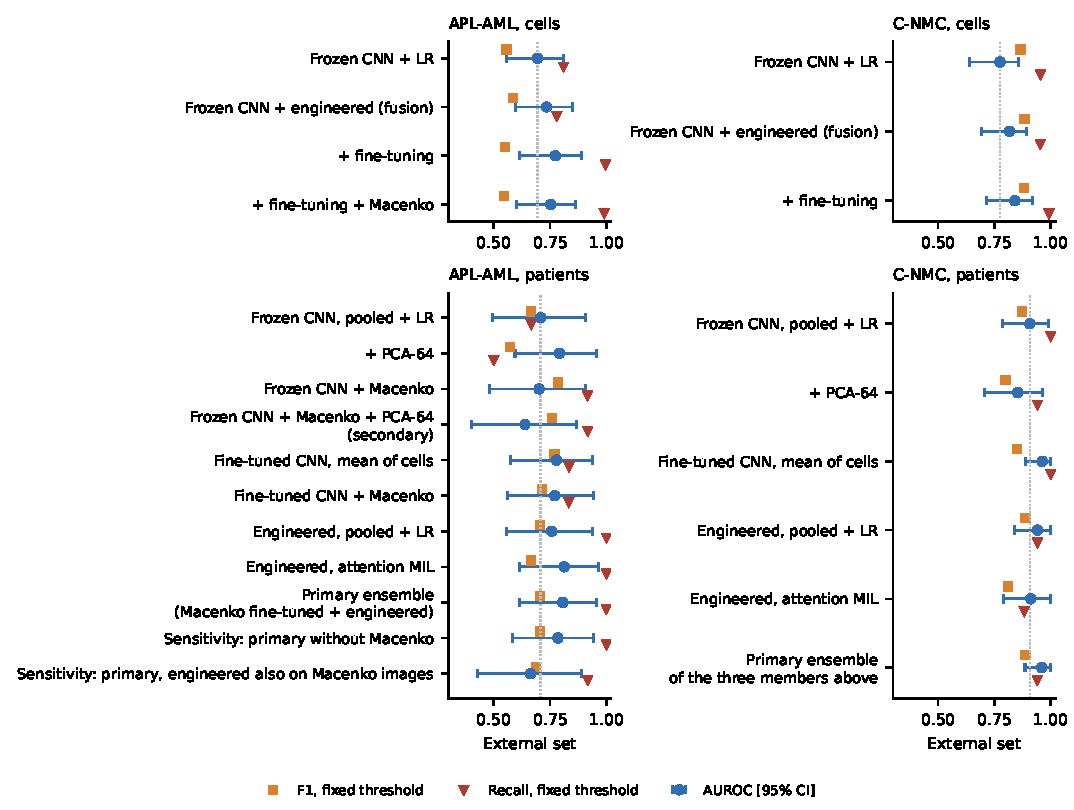
\includegraphics[width=\textwidth]{fig_ladder.pdf}
\caption{Effect of each added component on new patients (external sets): AUROC, F1 score and recall at the operating point fixed on development data, for cells and patients on both datasets.}
\label{fig:ladder}
\end{figure*}

\begin{table*}[!t]
\centering
\caption{Performance and complexity on APL-AML (24 external patients). Time per patient assumes 500 cells on our CPU (2 vCPUs): Macenko normalization 0.071 s, CNN forward pass 0.051 s and engineered features 0.038 s per cell; classifier times are measured. Storage: bytes kept per cell after feature extraction. Parameters and training time refer to the patient-level classifier (including PCA fitting).}
\label{tab:tradeoff}
\setlength{\tabcolsep}{3pt}
\resizebox{\textwidth}{!}{%
\begin{tabular}{lccccccccccc}
\toprule
 & \multicolumn{7}{c}{Performance (external, fixed threshold)} & \multicolumn{4}{c}{Complexity} \\
\cmidrule(lr){2-8}\cmidrule(lr){9-12}
Pipeline & AUROC & Acc. & Recall & Missed & Spec. & F1 & NPV & Storage/cell & Parameters & Training (s) & Time/patient (s) \\
\midrule
Primary: Macenko + fine-tuned CNN + engineered, ensemble & 0.806 & 0.58 & 1.00 & 0/12 & 0.17 & 0.71 & 1.00 & 5,492 B & 4,038,033 & 631.00 & 80 \\
Macenko + frozen CNN, no PCA & 0.701 & 0.75 & 0.92 & 1/12 & 0.58 & 0.79 & 0.88 & 5,120 B & 6,401 & 0.26 & 61 \\
Secondary: Macenko + frozen CNN + PCA-64 & 0.639 & 0.71 & 0.92 & 1/12 & 0.50 & 0.76 & 0.86 & 256 B & 321 & 6.15 & 61 \\
\bottomrule
\end{tabular}}
\end{table*}

\subsection{Replication on a Second Dataset}
\label{sec:cnmc}
Table~\ref{tab:cnmc}b repeats the patient-level experiment on C-NMC subjects (T5). All six models ranked the 31 external subjects well (AUROC 0.853--0.941), and engineered features again ranked best, both with pooled statistics (0.941, 95\% CI 0.840--1.000) and with attention MIL (0.912). In the feature-engineering experiments, engineered features alone reached 0.954--0.958 and their fusion with PCA-32 embeddings 0.966, whereas PCA alone lowered performance (Section~\ref{sec:pca}). Unlike on APL-AML, the operating point fixed on development data transferred: every model detected at least 15 of the 17 ALL subjects, three of the six detected all of them, and the pooled models detected 16 or 17 at specificities of 0.71--0.79. The contrast between the two datasets is instructive. On C-NMC the external fold is a random subject-disjoint split of the same collection, whereas the APL-AML Validation cohort was diagnosed later and differs in stain, cell counts and class balance; this suggests that the temporal shift, rather than the models, broke the threshold.

\begin{table*}[!t]
\centering
\caption{Replication on the second dataset, C-NMC 2019 (ALL vs.\ normal B cells; development: official folds 0--1, 42 subjects; external: fold 2, 31 unseen subjects, 17 with ALL). Same features, models, protocol and operating-point rule as for APL-AML. Leakage: image-level minus subject-grouped CV AUROC; shift: grouped CV minus external AUROC.}
\label{tab:cnmc}
\setlength{\tabcolsep}{3.5pt}
\resizebox{\textwidth}{!}{%
\begin{tabular}{llcccccccc}
\toprule
\multicolumn{10}{l}{\emph{(a) Cell level: every cell carries its subject's diagnosis (mean of 3 seeds)}} \\
Model & & Image CV & Grouped CV & External [95\% CI] & Recall & Spec. & F1 & Leakage & Shift \\
\midrule
Engineered + LR & & 0.933 & 0.864 & 0.840 [0.730, 0.902] & 0.95 & 0.58 & 0.89 & +0.069 & +0.023 \\
EfficientNet-B0 + LR & & 0.912 & 0.834 & 0.775 [0.640, 0.859] & 0.96 & 0.43 & 0.87 & +0.079 & +0.059 \\
Fusion + LR & & 0.939 & 0.864 & 0.817 [0.692, 0.892] & 0.95 & 0.54 & 0.88 & +0.075 & +0.047 \\
\midrule
\multicolumn{10}{l}{\emph{(b) Subject level: is this subject's sample leukemic?}} \\
Representation & Aggregation & CV AUROC & & External [95\% CI] & Recall (missed) & Spec. & F1 & NPV & \\
\midrule
Engineered & Pooled + LR & 0.906 & & 0.941 [0.840, 1.000] & 0.94 (1/17) & 0.79 & 0.89 & 0.92 & \\
EfficientNet-B0 & Pooled + LR & 0.855 & & 0.920 [0.807, 0.992] & 0.94 (1/17) & 0.71 & 0.86 & 0.91 & \\
Fusion & Pooled + LR & 0.878 & & 0.929 [0.824, 0.996] & 1.00 (0/17) & 0.71 & 0.89 & 1.00 & \\
Engineered & Attention MIL & 0.881 & & 0.912 [0.791, 1.000] & 0.88 (2/17) & 0.64 & 0.81 & 0.82 & \\
EfficientNet-B0 & Attention MIL & 0.874 & & 0.853 [0.704, 0.963] & 1.00 (0/17) & 0.43 & 0.81 & 1.00 & \\
Fusion & Attention MIL & 0.887 & & 0.853 [0.696, 0.967] & 1.00 (0/17) & 0.57 & 0.85 & 1.00 & \\
\bottomrule
\end{tabular}}
\end{table*}

\subsection{Analysis With More Statistical Power}
\label{sec:pooled}
Table~\ref{S-tab:pooled} shows the pooled CV over all 106 APL-AML patients. With 34 APL patients in the test folds, several differences became significant. The unreduced EfficientNet-B0 embedding ranked patients best (AUROC 0.953, 95\% CI 0.898--0.989), better than engineered features with pooled statistics ($-0.059$, Holm-adjusted $p<0.05$) and better than the promyelocyte fraction used as a manual biomarker (0.677). PCA with 32 or 64 components did not change the ranking, whether the component scores were whitened ($-0.005$ and $-0.011$) or kept at their natural scale ($+0.000$ and $+0.006$), and 16 components lost signal ($-0.074$ and $-0.057$). Thresholds chosen inside each training fold transferred to the held-out folds (recall 0.89--1.00), which supports the interpretation that the failure on the Validation cohort reflects temporal shift. Because patients from both periods were mixed, this analysis does not measure transfer to a later cohort and should be read alongside, not instead of, the external results.


\subsection{Can a New Laboratory Restore the Operating Point?}
\label{sec:recal}
Table~\ref{S-tab:recal} and Fig.~\ref{fig:recal} simulate a laboratory that confirms $k$ local patients before deploying a model. Setting the threshold just below the lowest score of the $m=k/2$ local APL cases gave the same expected recall for every model, about $m/(m+1)$: 0.50 with one local APL case and 0.80 with four (Fig.~\ref{fig:recal}a). This follows from the exchangeability of the local and future APL scores and does not depend on how well the model ranks patients, so about 19 confirmed local APL cases are needed before such a threshold can be expected to reach a recall of 0.95. Combining the development threshold with the local cases---lowering it only when a local APL case would otherwise be missed---raised recall from 0.50 to 0.80 with eight local cases for the frozen CNN models whose development threshold had missed half of the APL patients, at the cost of specificity (from 0.67--0.92 down to 0.44--0.49; Fig.~\ref{fig:recal}b). Even then, the probability of missing at least one APL patient among the remaining 16 was 0.66--0.68. Decision curves at an APL prevalence of 10\% (Fig.~\ref{fig:recal}c) showed net benefits close to those of testing every patient at threshold probabilities up to 5\%, and a small positive benefit above that; at a 5\% threshold, the attention MIL and fine-tuned models gave net benefits of 0.072 and 0.059 against 0.053 for testing everyone.


\begin{figure*}[!t]
\centering
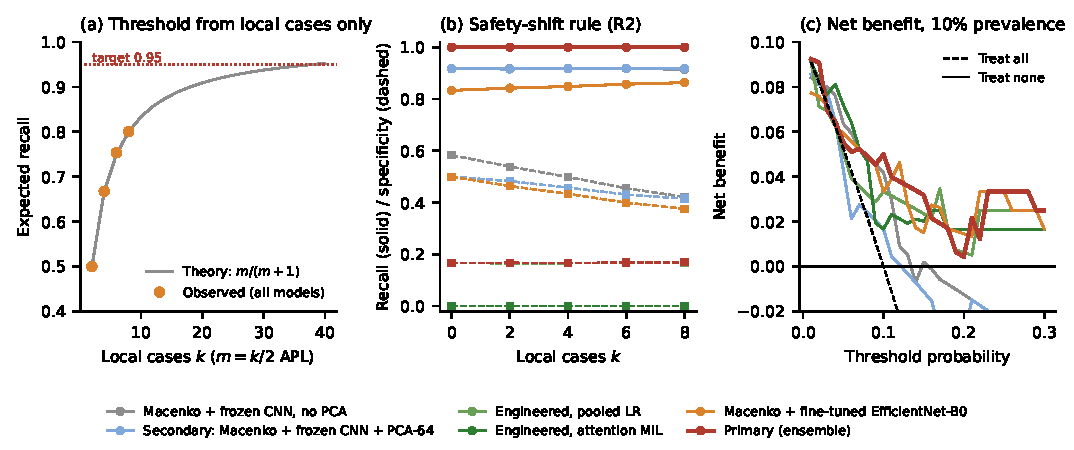
\includegraphics[width=\textwidth]{fig_recal.pdf}
\caption{Restoring the operating point at a new site (APL-AML Validation cohort). (a) Expected recall when the threshold is set just below the lowest score of $m=k/2$ local APL cases: observed values (all models give the same result) and the theoretical $m/(m+1)$. (b) Recall (solid) and specificity (dashed) when the development threshold is lowered only as far as needed to catch the local APL cases. (c) Decision curves at 10\% APL prevalence; dashed line: test every patient; horizontal line: test none.}
\label{fig:recal}
\end{figure*}

\subsection{Comparison With Existing Methods on the Same Cohort}
Table~\ref{tab:compare} compares our models with existing methods on the same patients. The original study reported a cell-level AUC of 0.743 in the later cohort \cite{sidhom2021apl}, and Manescu \emph{et al.} reported 0.96 with random three-fold CV \cite{manescu2023apl}; neither reported results at a fixed sensitivity. Because the protocols differ, we re-ran representative designs on the identical split with the same operating-point rule. The promyelocyte proportion, the biomarker used as comparator in \cite{sidhom2021apl}, reached an AUROC of 0.611, and a model on the full differential count reached 0.681. Averaging single-cell predictions per patient, as in \cite{sidhom2021apl}, reached 0.681--0.799 depending on the features, and the CNN-feature-plus-SVM design of \cite{kasim2025multiclass} reached 0.806. Our pre-specified primary pipeline reached 0.806 and missed no APL patient (specificity 0.17), as did the engineered pooled model on which it partly builds; attention MIL on engineered features ranked patients slightly better (0.812) but flagged every AML patient at the development threshold. With 24 external patients the confidence intervals of all learned models overlap; the clearest gains are over the manual biomarkers and in the number of missed APL patients, and the clearest difference between protocols is the gap between random CV (0.96) and temporal validation.

\begin{table*}[!t]
\centering
\caption{Comparison with existing methods on the same APL-AML cohort. Upper block: results as reported by the original studies, whose protocols differ from ours. Lower blocks: methods re-run on the identical split (trained on Discovery, tested once on the 24 Validation patients) with the same operating-point rule (sensitivity $\geq$ 0.95 on Discovery). The primary pipeline is compared with each of its members.}
\label{tab:compare}
\setlength{\tabcolsep}{3.5pt}
\begin{tabular}{p{4.6cm}p{3.6cm}ccccccc}
\toprule
Method & Evaluation & AUROC [95\% CI] & Recall (missed) & Spec. & F1 & NPV & Acc. \\
\midrule
\multicolumn{8}{l}{\emph{As reported in the literature}} \\
Single-cell CNN, Sidhom \emph{et al.} \cite{sidhom2021apl} & Temporal validation, cell level & 0.743 & -- & -- & -- & -- & -- \\
Annotation-free MIL, Manescu \emph{et al.} \cite{manescu2023apl} & Random 3-fold CV, patient level & 0.96 $\pm$ 0.02 & -- & -- & -- & -- & -- \\
Ten clinicians (reader study in \cite{sidhom2021apl}) & Same 24 Validation patients, smear images & \multicolumn{6}{l}{shown only graphically; the authors' MIL model was equivalent or better} \\
\midrule
\multicolumn{8}{l}{\emph{Re-run on the identical split (Validation cohort, patient level)}} \\
Promyelocyte proportion (biomarker in \cite{sidhom2021apl}) & Same protocol & 0.611 [0.371, 0.837] & 1.00 (0/12) & 0.00 & 0.67 & 0.00 & 0.50 \\
Differential count + LR (comparator in \cite{dasdelen2026caitomorph}) & Same protocol & 0.681 [0.437, 0.886] & 1.00 (0/12) & 0.08 & 0.69 & 1.00 & 0.54 \\
CNN features + SVM (design of \cite{kasim2025multiclass}) & Same protocol & 0.806 [0.615, 0.963] & 0.50 (6/12) & 0.75 & 0.57 & 0.60 & 0.62 \\
Single-cell classifier, engineered (design of \cite{sidhom2021apl}) & Same protocol & 0.681 [0.445, 0.908] & 0.75 (3/12) & 0.50 & 0.67 & 0.67 & 0.62 \\
Single-cell classifier, EfficientNet-B0 (design of \cite{sidhom2021apl}) & Same protocol & 0.799 [0.580, 0.972] & 0.58 (5/12) & 0.92 & 0.70 & 0.69 & 0.75 \\
Single-cell classifier, fusion (design of \cite{sidhom2021apl}) & Same protocol & 0.764 [0.536, 0.957] & 0.75 (3/12) & 0.75 & 0.75 & 0.75 & 0.75 \\
\midrule
\multicolumn{8}{l}{\emph{This work (pre-specified pipelines and their members)}} \\
\textbf{Primary pipeline (ensemble)} & Same protocol & 0.806 [0.615, 0.956] & 1.00 (0/12) & 0.17 & 0.71 & 1.00 & 0.58 \\
Member: engineered, pooled LR & Same protocol & 0.757 [0.555, 0.938] & 1.00 (0/12) & 0.17 & 0.71 & 1.00 & 0.58 \\
Member: engineered, attention MIL & Same protocol & 0.812 [0.614, 0.963] & 1.00 (0/12) & 0.00 & 0.67 & 0.00 & 0.50 \\
Member: Macenko + fine-tuned CNN & Same protocol & 0.771 [0.563, 0.941] & 0.83 (2/12) & 0.50 & 0.71 & 0.75 & 0.67 \\
Secondary pipeline (Macenko + frozen CNN + PCA-64) & Same protocol & 0.639 [0.400, 0.867] & 0.92 (1/12) & 0.50 & 0.76 & 0.86 & 0.71 \\
\bottomrule
\end{tabular}
\end{table*}

\subsection{Ablation and Interpretation}
Table~\ref{S-tab:ablation} and Fig.~\ref{S-fig:impact} show which engineered feature groups matter for blast detection. Removing the stain and color group cost $-0.034$ AUROC (95\% CI $-0.060$ to $-0.015$), chromatin texture $-0.012$ and the basophilic region $-0.005$; nuclear shape, local binary patterns and the nucleolus and granule proxies were redundant given the other groups. Temperature scaling fitted on Discovery left the external calibration error at 0.06--0.13 for cell-level models and 0.26--0.36 for patient-level models. Attention weights of the best patient-level model were highest for cells labeled as monocytes (2.5 times the average in AML patients and 2.8 times in APL patients) and lowest for smudge cells in AML patients (0.31 times the average); since monocytes are nearly absent in APL (Fig.~\ref{fig:dataset}b), the model appears to use monocyte-like cells as evidence against APL.




%======================================================================
\section{Discussion}
Four findings stand out. First, how a model is evaluated changes the reported number far more than how it is built. The same classifiers reached 88--95\% accuracy when cells of one patient could appear in training and test sets, but 69--90\% on patients they had never seen; the AUROC inflation was largest (up to 0.32) when cells carried their patient's diagnosis and smallest (at most 0.04) when the label described the cell itself. This held on two datasets from different laboratories and may explain why studies that held out whole subjects, such as the C-NMC challenge entries \cite{prellberg2019cnmc,mondal2021ensemble}, report F1 scores near 0.89 rather than near 1.0.

Second, the data decided which design choices helped. The exploratory analysis found a stain shift between the two APL-AML cohorts and none in C-NMC, and this one observation explained several results: stain normalization helped on APL-AML and slightly hurt on C-NMC; development thresholds transferred to the C-NMC external fold but not to the later APL cohort; and a test that asks whether cells can be traced to their cohort, which needs no labels from the new site, is a practical way to decide whether normalization is worth its cost. Among the modelling choices, fine-tuning the CNN was the only one that improved results on both datasets. PCA reduced the patient-level model 20-fold with a small loss in performance, which makes it a reasonable option when storage, memory or retraining effort matter, but not a way to gain accuracy; a common preprocessing default---standardizing each principal component---made its effect erratic. Nested early stopping and attention pooling did not improve on the simpler fixed settings, and early stopping was less stable because the inner validation sets were small; we report these negative results because they justify the settings we kept.

Third, ranking transferred better than decisions. On the later APL cohort the primary pipeline missed no APL patient but cleared only 2 of 12 AML patients, and every other model either missed patients or flagged most of the AML cohort. Our recalibration analysis sets a sobering bound for the obvious remedy: a threshold placed below the lowest of $m$ local positive cases has an expected recall of only $m/(m+1)$, whatever the model, so about 20 confirmed local cases are needed before a recall of 0.95 can be expected. For a condition in which a missed diagnosis can be fatal, a model like ours is best used to prioritize smears for urgent review, with its threshold confirmed on local cases.

Fourth, small external sets make honest reporting harder than it looks. With 24 external patients, AUROC confidence intervals spanned about $\pm0.18$, single folds of 16 patients varied by up to 0.25, and several apparent gains---PCA on the temporal test, Macenko on a subset---shrank or vanished with more data or a second dataset. Fixing the primary pipeline and the selection rules before the final analysis, and confirming every component on a second dataset and in pooled cross-validation, was what kept us from reporting them as methods.

This study has limitations. The two datasets differ in disease (APL vs.\ other AML; ALL vs.\ normal B cells), so the replication tests the evaluation principles and design choices rather than one clinical model across sites; an independent AML cohort with APL cases remains to be tested. The external sets are small (24 patients and 31 subjects), and the preprocessing comparison used a subset that included the APL-AML Validation patients, which we disclose; the final pipelines were fixed before their full evaluation. Cell labels in APL-AML come from an analyzer verified by an operator rather than from expert consensus, and our cytoplasm features rely on proxies. Fine-tuning was partial (the last two stages), limited to 5,000 cells per fold and run with one seed on a CPU; stain augmentation, full fine-tuning on a GPU and hematology foundation models such as DinoBloom \cite{koch2024dinobloom}, whose weights we could not obtain in our computing environment, may perform better.

%======================================================================
\section{Conclusion}
Reported accuracy for leukemia detection from blood smears depends strongly on how the evaluation is set up. Across two public datasets, splitting cells instead of patients inflated performance substantially when cells carried the patient's diagnosis. Building the pipeline step by step from the data---stain normalization only where a shift was found, fine-tuned and interpretable features, and pre-specified combination and thresholds---gave a model that missed no APL patient in a later cohort and 1 of 17 leukemic subjects in a second dataset, while showing that PCA trades a little performance for a much smaller model and that early stopping and attention pooling added nothing at this data size. Decision thresholds remained the weak point under temporal shift, and restoring them locally requires about 20 confirmed positive cases. We recommend that studies in this area split data by patient, analyze the data before choosing preprocessing, test on more than one external set, report recall, missed cases, specificity, F1 score, NPV and calibration at a pre-specified operating point, and report the computational cost of every component.

\section*{Data and Code Availability}
The APL-AML cohort is available at \url{https://github.com/sidhomj/DeepAPL}. Code, split files, label maps and per-model outputs are released at \url{https://github.com/Sherif-Hussein/leukemia-leakage-benchmark}. Reporting follows TRIPOD+AI \cite{collins2024tripodai}.

\bibliographystyle{IEEEtran}
\bibliography{refs}

\end{document}
